\documentclass[12pt,a4paper]{article}
\usepackage[utf8]{inputenc}
\usepackage[T1]{fontenc}
\usepackage{graphicx}
\usepackage{tikz-feynman}
\usepackage{xcolor,simpler-wick}
\usepackage{empheq}
\usepackage{braket}
\usepackage{subcaption}
\usepackage{physics}
\usepackage{amsmath,amssymb,amsthm}
\usepackage[a4paper]{geometry} % per modificare le dimensioni e i margini del documento
\usepackage{appendix}
\newgeometry{top=2cm, bottom=1.8cm, left=2cm, right=2cm}
% Local fallback for the 'wick' package (not available offline):
% marks a contracted field with an over-arc.
\renewcommand{\c}[1]{\overset{\frown}{#1}}
 
\title{Linearized Gravity and QFT Connection}
\author{Matteo Falasca}
\date{March 2026}

\begin{document}
\maketitle

\begin{abstract}
In this work we present a modern and self‑contained review of the quantum theory of linearized gravity, starting from General Relativity and progressing to its canonical quantization. We then develop a minimal yet operational framework to describe gravitationally induced decoherence, deriving the master equation governing open quantum systems in the weak‑field regime.\end{abstract}

% ====================================================================
\section{Introduction to Linearized Gravity}
% ====================================================================

In GR, we speak of linearized gravity whenever our metric is almost flat. Technically, we can expand our metric around flat space:
\[
g_{\mu\nu} = \eta_{\mu\nu} + h_{\mu\nu}, \qquad |h_{\mu\nu}| \ll 1
\]
where $|h|$ is much smaller than 1.
We will use the mostly negative flat space metric.

\subsubsection*{Validity}

$h$ is different from observer to observer. Under an infinitesimal coordinate transformation, we have a family of diffeomorphisms of linearized metrics.
\[
h_{\mu\nu} \to h_{\mu\nu} + \partial_\mu \xi_\nu + \partial_\nu \xi_\mu, \qquad |\partial_\mu \xi_\nu| \ll 1
\]

It's important to notice that boost and translation around all space don't led to
any change in the metric tensor. 
The only coordinate changes are local ones, which are slowly varying in space and time.

The linearized metric behaves as a tensor under Lorentz transformations. In this sense, we can assume linearized gravity as Covariant, as long as we take slowly varying frame of reference compared to a valid one. \\
The complete diffeomorfism expansion around flat metric won't be much important for our calculations, but will be mathematically consistent in the next sections.

\subsection*{Equations of Motion}
Starting from the GR EoM
\[
R_{\mu\nu} - \frac{1}{2}g_{\mu\nu}R = 8\pi G\, T_{\mu\nu}
\]
it's first order terms in $h_{\mu\nu}$ are easily calculated by defining the trace and the trace-less perturbation:
\[
h = \eta^{\mu\nu} h_{\mu\nu}
\]
\[
\bar{h}_{\mu\nu} = h_{\mu\nu} - \frac{1}{2}\eta_{\mu\nu} h
\]
and then by computing the linearized Ricci and Einstein tensor:
\[
R_{\mu\nu}^{(1)} = \frac{1}{2}\left( -\Box h_{\mu\nu} - \partial_\mu \partial_\nu h + \partial^\lambda \partial_\mu h_{\nu\lambda} + \partial^\lambda \partial_\nu h_{\mu\lambda} \right)
\]
\[
G_{\mu\nu}^{(1)} = -\frac{1}{2}\left( \Box \bar{h}_{\mu\nu} + \eta_{\mu\nu} \partial^\lambda \partial^\rho \bar{h}_{\lambda\rho} - \partial^\lambda \partial_\mu \bar{h}_{\nu\lambda} - \partial^\lambda \partial_\nu \bar{h}_{\mu\lambda} \right)
\]

Due to diffeomorphism invariance, the metric perturbation contains redundant degrees of freedom. In 4D this reduces to 2 physical DoF in vacuum (gravitational waves), 6 with sources. This is well explained in Maggiore and confirmed by the Hamiltonian analysis in flat space via first-class constraints removing the unphysical modes.


 
\subsection*{Harmonic Gauge}

This gauge is covariant and expressed as:
\begin{equation}
\boxed{\partial^\mu\bar{h}_{\mu\nu} = 0}
\label{eq:DD}
\end{equation}
We can always reach this, via a gauge transformation made b
from a proper infinitesimal coordinate transformation:
\[
\partial^\mu \bar{h}_{\mu\nu} \to \partial^\mu \bar{h}_{\mu\nu} - \Box \xi_\nu
\]
Looking at the Eom, they reduce to:
\begin{equation}
\Box \bar{h}_{\mu\nu} = \frac{-16\pi G}{c^4}\, T_{\mu\nu}
\label{eq:EoM}
\end{equation}
which leads immediately to:
\[
\partial^\mu T_{\mu\nu} = 0
\]

And outside the source to:
\begin{equation}
    \boxed{
\Box \bar{h}_{\mu\nu} = 0
}\label{eq:EoM2}
\end{equation}

\subsection*{TT Gauge}

De Donder gauge ($\ref{eq:DD}$) is not broken by a coordinate 
change such that $\Box \xi_\mu = 0$. Then $\xi$ definition can be 
extended at: 
\begin{align}
    \Box \xi_{\mu\nu}=0 \quad \text{s.t.} \quad \xi_{\mu\nu} \equiv \partial_\mu\xi_\nu + \partial_\nu \xi_\mu -\eta_{\mu\nu}\partial_\rho\xi^\rho
\end{align}

This allows to have on shell solutions such that ($\ref{eq:EoM2}$)
and:

\begin{align}\label{TTC}
\boxed{
    h^{0\mu}=0 \qquad h^i_i=0 \qquad \partial_i h^{ij}=0
}
\end{align}
In this framework the EoM are:
\[
\boxed{\Box h_{\mu\nu}=0}
\]

Now, we want to express wave solutions.
 Denoting by $(a,b)$ the plane perpendicular to the wave:
\[
h^{\mathrm{TT}}_{ij}(t,z) =
\begin{pmatrix}
h_+ & h_\times \\
h_\times & -h_+
\end{pmatrix}
\cos[\omega(t - z/c)]
\]





\newpage
\section{Field Action}
In \textit{GR}, the \textit{covariance principle} requires the action to be invariant under coordinate changes. Since $\sqrt{-g}$ and $d^4x$ each produce a Jacobian factor under a change of coordinates, and the two cancel, covariance can be achieved by writing action in the form:
\[
S = \int d^4x \, \sqrt{-g}\, \bigl[ \mathcal{L}_{HE} + \mathcal{L}_M \bigr]
\]

We take $\mathcal{L}_{HE} = \frac{1}{16 \pi G} R$. Higher-curvature proposals exist, but we will not consider them here.



\subsection*{Expansion of the building blocks}
 
Set $g_{\mu\nu} = \eta_{\mu\nu} + \kappa h_{\mu\nu}$, $h \equiv h^\mu_\mu$. Everything geometric ($g^{\mu\nu}$, $\sqrt{-g}$, $\Gamma^\lambda_{\mu\nu}$, $R$) is an infinite series in $h$; we keep terms up to $O(h^3)$, which is what's needed for the 3-graviton vertex.
 
Inverse metric, order by order (from $g^{\mu\nu}g_{\nu\rho}=\delta^\mu_\rho$):
\[
g^{\mu\nu} = \eta^{\mu\nu} - \kappa h^{\mu\nu} + \kappa^2 h^{\mu\lambda}h^\nu_\lambda - \kappa^3 h^{\mu\lambda}h_\lambda^\alpha h_\alpha^\nu + \cdots
\]
 
Determinant, using $\ln\det g = \mathrm{tr}\ln g$:
\[
\det(g_{\mu\nu}) = -1 - \kappa h + \tfrac12\kappa^2(h^\mu_\rho h^\rho_\mu - h^2) + \tfrac16\kappa^3(-2h^\mu_\rho h^\rho_\gamma h^\gamma_\mu + 3h\,h^\mu_\rho h^\rho_\mu - h^3)
\]
so that
\[
\sqrt{-g} = 1 + \frac{\kappa}{2}h + \frac{\kappa^2}{8}(h^2 - 2h^\mu_\rho h^\rho_\mu) + \frac{\kappa^3}{48}(h^3 - 6h\,h^\mu_\rho h^\rho_\mu + 8h^\mu_\rho h^\rho_\gamma h^\gamma_\mu)
\]

We have obtained it using '$\ln(\det(-g))=\text{tr} (\ln(-g))$' and
\[
\det g_{\mu\nu}
= \det\eta_{\mu\alpha}\det(\delta^\alpha_\nu+h^\alpha_\nu)
= (-1)\det(\mathbf{1+H})
\]

Then by expanding the logarithm and the exponential.

 
Affine connection, directly from its definition and the two series above:
\[
\Gamma^\lambda_{\mu\nu} = \frac{\kappa}{2}\bigl(\eta^{\lambda\sigma} - \kappa h^{\lambda\sigma} + \kappa^2 h^{\lambda\alpha}h_\alpha^\sigma\bigr)\bigl(\partial_\mu h_{\sigma\nu} + \partial_\nu h_{\sigma\mu} - \partial_\sigma h_{\mu\nu}\bigr)
\]
 
Ricci scalar:
\[
R = g^{\mu\nu}\bigl[\partial_\nu \Gamma^\lambda_{\mu\lambda} - \partial_\lambda\Gamma^\lambda_{\mu\nu} + \Gamma^\tau_{\mu\lambda}\Gamma^\lambda_{\tau\nu} - \Gamma^\tau_{\mu\nu}\Gamma^\lambda_{\tau\lambda}\bigr]
\]

 
\vspace{1cm}
Therefore, we can expand the Hilbert-Einstein action and collect everything into 
powers of $\kappa$:  $$\sqrt{-g}\,\mathcal{L}_{HE} = \frac{2}{\kappa^2}\sqrt{-g}R \equiv \mathcal{L}_g^0 + \mathcal{L}_g^1 + \mathcal{L}_g^2 + \cdots$$
and: $$\sqrt{-g}\,\mathcal{L}_{M}  \equiv \mathcal{L}_M^0 + \mathcal{L}_M^1 + \mathcal{L}_M^2 + \cdots$$
\\where we have that \underline{$\mathcal{L}^N = \kappa^N \;\,\mathclap{F}\,\;(\varphi, \partial \varphi)$}.


\subsection*{Linearized Gravity: Free action}
After rescaling, the leading order
of Hilbert-Einstein action is called Pauli Fierz action,
which resembles the free field lagrangian. 
\begin{align}
S^{(2)}_{HE}= \frac{1}{2 \kappa^2} \int d^4x \bigl[
&\partial_\mu h_{\alpha\beta}\partial^\mu h^{\alpha\beta}
- \partial_\mu h \partial ^\mu h \nonumber \\
&+ 2\partial_\mu h^{\mu\nu}\partial_\nu h
-2\partial_\mu h^{\mu\nu}\partial_\rho h^\rho_\nu
\bigr]
\end{align}


\begin{equation}
\mathcal{L}^0_g\equiv
-\partial_\rho h_{\mu\nu}\partial^\rho h^{\mu\nu}
+2\partial_\rho h_{\mu\nu}\partial^\nu h^{\mu\rho}
-2\partial_\nu h^{\mu\nu}\partial_\mu h
+\partial_\mu h\partial^\mu h
\end{equation}
 

 
\subsection*{Self interaction: Cubic term}

 
Order $k^1$: the three-graviton self-interaction, already reduced (STRONGLY IMPOSED DD GAUGE, Illegal?
, and integration by parts) to 6 contributions (Choi). 

\begin{align}
S^{(3)}_{HE} = \int d^4x\, \mathcal{L}_g^1, \qquad
\mathcal{L}_g^1 =\;\kappa  \Bigl[
&\frac{1}{2} h_\beta^\alpha \partial^\mu h_\alpha^\beta \partial_\mu h
- \frac{1}{2} h_\beta^\alpha \partial_\alpha h_\nu^\mu \partial^\beta h_\mu^\nu
- h_\beta^\alpha \partial_\mu h_\alpha^\nu \partial^\mu h_\nu^\beta \nonumber \\
&+ \frac{1}{4} h\, \partial^\beta h_\nu^\mu \partial_\beta h_\mu^\nu
+ h_\mu^\beta \partial_\nu h_\beta^\alpha \partial^\mu h_\alpha^\nu
- \frac{1}{8} h\, \partial^\nu h\, \partial_\nu h \Bigr]
\end{align}



\subsection*{Linearized action: Interaction terms}
We are interested in interaction between matter fields and linearized gravity. To analyse this in a simpler way, we will suppose that mass is described by a Klein-Gordon Lagrangian, because interaction structure is independent of the type of field we are using. Expanding the metric and its determinant into the matter part of the action, we will get a free matter contribute and various terms containing information about the gravity interacting with the matter:
\[
\int d^4x \,\sqrt{-g} \; \mathcal{L}_M
= S_M^{(0)} + S_M^{(1)} + S_M^{(2)} + \mathcal{O}(h^3)
\]


\vspace{1em}
\textsc{\textbf{Interaction terms:}}
The zeroth-order term is, as expected, the free field action in flat space (ordine $\kappa^0$):
\[
\boxed{
S_M^{(0)}
= \int d^4x \Big(\frac{1}{2}\eta^{\mu\nu}\partial_\nu \phi \partial_\mu \phi - \frac{m^2}{2}\Big)}
\]

The first-order vertex couples $h_{\mu\nu}$ to the flat-space stress-energy tensor. Un $h$, quindi ordine $\kappa^1$:
\[
\boxed {
S_M^{(1)} = -\frac{\kappa}{2} \int d^4x \, h^{\mu\nu}T_{\mu\nu}
=
-\frac{\kappa}{2} \int d^4x \, h^{\mu\nu}
\left[
\partial_\mu \phi\, \partial_\nu \phi
- \eta_{\mu\nu}\left(\frac12 \partial_\rho \phi\, \partial^\rho \phi - \frac12 m^2 \phi^2\right)
\right]
}
\]

The second-order vertex takes the form (due $h$, ordine $\kappa^2$):
\begin{align}
\boxed{
S^{(2)}=\kappa^2\int d^4x \Biggl\{
\frac{1}{4}\bigl(\frac12h^2-h_{\alpha\beta}h^{\alpha\beta}\bigr)\mathcal{L}_M \nonumber - \frac{hh^{\mu\nu}}{4}\partial_\mu\phi\partial_\nu\phi \nonumber + \frac{1}{2}h^{\mu\alpha}h_\alpha^\nu \partial_\mu\phi\partial_\nu\phi
\Biggr\}
}
\end{align}

\textsc{Indexed are moved by the flat metric for convention}
\vspace{1cm}



\newpage
\section{Lagrangians in De Donder gauge}
 
Collecting the results above, the full action up to the orders considered, expressed in the harmonic (De Donder) gauge, reads:
(In the next chapter we will explain what De Donder gauge means for the free Lagrangian. Meanwile, for 
the self interacting one, we followed literature imposing the Harmonic condition on the field exactly.) 
\[
\boxed{
\begin{aligned}
\mathcal L_g^{(0)}
&=
\frac{1}{2}
\left[
\partial_\mu h_{\alpha\beta}\partial^\mu h^{\alpha\beta}
-\frac12
\partial_\mu h\,\partial^\mu h
\right]
\qquad (\kappa^0)
\\[0.5cm]
\mathcal L_g^{(1)}
&=
\kappa\Biggl[
\frac12 h_\beta^\alpha
\partial^\mu h_\alpha^\beta
\partial_\mu h
-\frac12 h_\beta^\alpha
\partial_\alpha h_\nu^\mu
\partial^\beta h_\mu^\nu
-h_\beta^\alpha
\partial_\mu h_\alpha^\nu
\partial^\mu h_\nu^\beta
\\
&\quad
+\frac14 h
\partial^\beta h_\nu^\mu
\partial_\beta h_\mu^\nu
+h_\mu^\beta
\partial_\nu h_\beta^\alpha
\partial^\mu h_\alpha^\nu
-\frac18 h
\partial^\nu h
\partial_\nu h
\Biggr]
\qquad (\kappa^1)
\\[0.5cm]
\mathcal L_M^{(0)}
&=
\frac12\partial_\mu\phi\,\partial^\mu\phi
-\frac12m^2\phi^2
\qquad (\kappa^0)
\\[0.5cm]
\mathcal L_M^{(1)}
&=
-\frac{\kappa}{2} h^{\mu\nu}
\left[
\partial_\mu\phi\,\partial_\nu\phi
-\eta_{\mu\nu}
\left(
\frac12\partial_\rho\phi\,\partial^\rho\phi
-\frac12m^2\phi^2
\right)
\right]
\qquad (\kappa^1)
\\[0.5cm]
\mathcal L_M^{(2)}
&=
\kappa^2\left[
\frac14
\left(
\frac12h^2-h_{\alpha\beta}h^{\alpha\beta}
\right)
\mathcal L_M^{(0)}
-\frac14 h\,h^{\mu\nu}\partial_\mu\phi\,\partial_\nu\phi
+\frac12h^{\mu\alpha}h_\alpha^\nu
\,\partial_\mu\phi\,\partial_\nu\phi
\right]
\qquad (\kappa^2)
\end{aligned}
}
\]
 
$\mathcal{L}_g^{(1)}$  is obtained imposing strongly Harmonic condition, it would be different otherwise.
De Donder projector is:
\[
P_{\mu\nu,\alpha\beta}^{\mathrm{H}}
=
\frac12
\left(
\eta_{\mu\alpha}\eta_{\nu\beta}
+\eta_{\mu\beta}\eta_{\nu\alpha}
-\eta_{\mu\nu}\eta_{\alpha\beta}
\right)
\]
 
\subsection{Lagrangians in TT gauge}
By projecting the action in TT gauge, we have that the free graviton action reduces to:
\[
\boxed{
\begin{aligned}
\mathcal{L}^{(2)}_{HE} &= \frac{1}{2} \partial_k h_{ij}\,\partial^k h^{ij} &&(\kappa^0)\\[0.3cm]
\mathcal{L}_{I}^{(1)} &= -\frac{\kappa}{2} h^{ij}\,\partial_i\phi\,\partial_j\phi &&(\kappa^1)\\[0.3cm]
\mathcal{L}^{(2)}_{I} &= \kappa^2 \Biggl[
\frac{1}{4} h_{ij}h^{ij}
\left( \frac{1}{2}\partial_\rho\phi\,\partial^\rho\phi
- \frac{1}{2}m^2\phi^2 \right)
+ \frac{1}{2} h^{ij}h_{j}^{k}
\,\partial_i\phi\,\partial_k\phi\Biggr] &&(\kappa^2)\\
\mathcal{L}_g^{(1)} &= \kappa \Biggl[
-\frac12 h_l^k\,\partial_k h_j^i\,\partial^l h_i^j
- h_l^k\,\partial_i h_k^j\,\partial^i h_j^l
+ h_i^l\,\partial_j h_l^k\,\partial^i h_k^j
\Biggr]
&&(\kappa^1)\\
\end{aligned}
}
\]

The projector onto the TT gauge is:
\begin{equation}
\Lambda_{ij,kl}(\hat{n}) = \frac{1}{2}\left(P_{ik}P_{jl} + P_{il}P_{jk} - P_{ij}P_{kl}\right)
\label{TTP}    
\end{equation}

with
\begin{equation}
P_{ij}=\delta_{ij}-n_in_j
\label{TTPs}    
\end{equation}



\newpage
\section{Hamiltonian}
\subsection{Free hamiltonian}
The full hamiltonian reads as:
\[
\hat{H} = \hat{H}_0^{\mathrm{KG}} + \hat{H}_0^{\mathrm{PF}} + \hat{H}^I + \hat{H}^{SI}
\]

Conjugate momenta of the free fields:
\begin{equation}
    \label{piphi}
    \boxed{\pi_\phi=\dot\phi}
\end{equation}
\begin{equation}\label{pih}
    \boxed{\pi^{\mu\nu}=(\dot h^{\mu\nu}-\tfrac12\eta^{\mu\nu}\dot h)}
\end{equation}

Free Hamiltonians:
\begin{equation} \boxed{
    \mathcal{H}_0^{\mathrm{KG}} = \frac{1}{2}\Bigl(\pi_\phi^2 + (\vec{\nabla}\phi)^2 + m^2\phi^2\Bigr)
}\end{equation}
\begin{equation}\label{HPF}\boxed{
    \mathcal{H}_0^{\mathrm{PF}} = \frac{1}{2}\Bigl(\pi_{\mu\nu}\pi^{\mu\nu} - \tfrac12\pi^2
    + (\vec\nabla h_{\mu\nu})\cdot(\vec\nabla h^{\mu\nu}) - \tfrac12(\vec\nabla h)^2\Bigr)
}\end{equation}


\subsection{Hamiltonian in Interaction Picture}
To compute scattering matrix, we are interested in the hamiltonian
representetions in the interaction picture.
To do so, we will employ \eqref{pih} and \eqref{piphi}, imposing that the canonically
conjugate fields in the interaction picture obey the same equations of the noninteracting case,
since the interaction picture was introduced in order to have field operators satisfying the dynamics
of free fields:

\begin{equation}
    \label{piIphi}
    \boxed{\pi_\phi^I=\dot\phi^I}
\end{equation}
\begin{equation}\label{piIh}
    \boxed{\pi^{I\mu\nu}=(\dot h^{I\mu\nu}-\tfrac12\eta^{\mu\nu}\dot h^I)}
\end{equation}

Then, we transform the operators according to:

\begin{equation}
    \hat{O}^I(t)=\hat{U}(t)\hat{O}^H(t)\hat{U}^{-1}(t)
\end{equation}

What's interesting is that, by doing this, we recover that for the \textit{interaction
terms}:

\begin{equation}\label{HIN}
    \mathcal{\hat{H}}^I=-\mathcal{\hat{L}}^I[\Phi^I] + \mathcal{N}
\end{equation}

Where $\mathcal{N}$ is a "normal-dependent" term. To say, a term that depends on the
unit normal $n^\mu$ to the space-like hyper surface on which we quantize, which for the
equal-time condition $x_0=x_0'$ is $n^\mu=(1,\vec{0})$.
One way to see this is by performing the explicit transformation of all the
lagrangians, for which we get \eqref{HIN} directly, just as in the scalar QED case.

The point is that now $\mathcal{\hat{H}}^I$ contains
many terms that break covariance, which, to say, come from all the terms like $\pi\dot{\Phi}$
in the Legendre transform.
The point is that, like in scalar QED, all those terms cancel out due to the derivatives
of the two point function. As a matter of fact, we can see that, if on one hand a single
time derivative acting on fields that have to be contracted gives no extra term (since
$[\Phi(\vec x,t),\Phi(\vec y,t)]=0$), when
two or more time derivatives act on a two point function in the scattering matrix, we have
that there appears a contact term:
\begin{equation}\label{contact}
    \partial_0^x\partial_0^y\,T\{\phi^I(x)\phi^I(y)\}
    = T\{\dot\phi^I(x)\dot\phi^I(y)\} + i\,\delta^{(4)}(x-y)
\end{equation}
which acts both on the tensorial part of the
fields both on its scalar part. The point is that this leds to having contact terms, that
in theory cancel out the normal-dependent term that had just shown up in the Hamiltonian.
This conclusion holds true in general, and to show it, it would be enough to show it at
our first order interaction, since then we could show that every feynmann diagram which are of
the same order, contain subgraphs which are the same order and which their
contributions combine to cancel out each other normaldependent term.

However this may be pretty tedious to show in our gravitational case, so we stop at the Scalar
QED level with the analogy and we refer to (Rohrlich1950) and to (Matthews1949,BernardDuncan1975) to justify that we will just do the following:

\begin{itemize}
    \item Use $\mathcal{\hat{H}}^I=-\mathcal{\hat{L}}^I[\Phi^I]$ (drop $\mathcal{N}$)
    \item Use the \textit{modified time-ordered product $T^*$}, defined so as to commute
    with all derivatives: \begin{equation}\label{Tstar}
        T^*\{\partial_{\mu_1}\Phi(x_1)\cdots\partial_{\mu_n}\Phi(x_n)\}
        \equiv \partial_{\mu_1}^{x_1}\cdots\partial_{\mu_n}^{x_n}\,
        T\{\Phi(x_1)\cdots\Phi(x_n)\}
    \end{equation}
    so that the contact terms in \eqref{contact} are reabsorbed and the propagators are
    the naive covariant ones.
\end{itemize}

To summarize: \textit{in scalar QED the normal-dependent terms can simply be ignored in
the perturbation expansion. We use the same results to
do the same in our graviton case.}

\newpage
\section{Interaction Hamiltonians in the Interaction Picture}

Applying the prescription established above, the interaction Hamiltonian densities are
obtained from the Lagrangians of the previous section as
\begin{equation}\label{HIrecipe}
    \mathcal{\hat{H}}^{I}=-\mathcal{\hat{L}}^{I}[\Phi^{I}]+\mathcal{N},
\end{equation}
all fields being interaction-picture fields obeying \eqref{piIphi} and \eqref{piIh}.

\subsection{De Donder gauge}

\[
\boxed{
\begin{aligned}
\mathcal H_g^{(1)}
&=
-\kappa\Biggl[
\frac12 h_\beta^\alpha
\partial^\mu h_\alpha^\beta
\partial_\mu h
-\frac12 h_\beta^\alpha
\partial_\alpha h_\nu^\mu
\partial^\beta h_\mu^\nu
-h_\beta^\alpha
\partial_\mu h_\alpha^\nu
\partial^\mu h_\nu^\beta
\\
&\quad
+\frac14 h
\partial^\beta h_\nu^\mu
\partial_\beta h_\mu^\nu
+h_\mu^\beta
\partial_\nu h_\beta^\alpha
\partial^\mu h_\alpha^\nu
-\frac18 h
\partial^\nu h
\partial_\nu h
\Biggr]
\qquad (\kappa^1)
\\[0.5cm]
\mathcal H_M^{(1)}
&=
+\frac{\kappa}{2} h^{\mu\nu}
\left[
\partial_\mu\phi\,\partial_\nu\phi
-\eta_{\mu\nu}
\left(
\frac12\partial_\rho\phi\,\partial^\rho\phi
-\frac12m^2\phi^2
\right)
\right]
\;=\;\frac{\kappa}{2}h^{\mu\nu}T_{\mu\nu}
\qquad (\kappa^1)
\\[0.5cm]
\mathcal H_M^{(2)}
&=
-\kappa^2\left[
\frac14
\left(
\frac12h^2-h_{\alpha\beta}h^{\alpha\beta}
\right)
\mathcal L_M^{(0)}
-\frac14 h\,h^{\mu\nu}\partial_\mu\phi\,\partial_\nu\phi
+\frac12h^{\mu\alpha}h_\alpha^\nu
\,\partial_\mu\phi\,\partial_\nu\phi
\right]
+\mathcal{N}_M^{(2)}
\qquad (\kappa^2)
\end{aligned}
}
\]

\subsection{TT gauge}

\[
\boxed{
\begin{aligned}
\mathcal{H}_{M}^{(1)} &= +\frac{\kappa}{2} h^{ij}\,\partial_i\phi\,\partial_j\phi &&(\kappa^1)\\[0.3cm]
\mathcal{H}^{(2)}_{M} &= -\kappa^2 \Biggl[
\frac{1}{4} h_{ij}h^{ij}
\left( \frac{1}{2}\partial_\rho\phi\,\partial^\rho\phi
- \frac{1}{2}m^2\phi^2 \right)
+ \frac{1}{2} h^{ij}h_{j}^{k}
\,\partial_i\phi\,\partial_k\phi\Biggr] &&(\kappa^2)\\[0.3cm]
\mathcal{H}_g^{(1)} &= -\kappa \Biggl[
-\frac12 h_l^k\,\partial_k h_j^i\,\partial^l h_i^j
- h_l^k\,\partial_i h_k^j\,\partial^i h_j^l
+ h_i^l\,\partial_j h_l^k\,\partial^i h_k^j
\Biggr]
&&(\kappa^1)\\
\end{aligned}
}
\]


\newpage
\section{Quantization of the Linearized Gravity Field}
\subsection{Introduction}

In the quantization of spin-1 fields, such as the photon field, in the context of the canonical formalism, we can find cases where the $0$-component of the potential $A^0(x)$ has no conjugate field of its own, since the Lagrangian does not depend on its time derivative. This has not turned out to be a problem, because its time part could be expressed as a quantity depending on the other fields, and it was enough to quantize the spatial part. Contrary to superficial evidence, this procedure was relativistically covariant (Greiner). In particular, in the case of QED, the vector field $A^\mu$ has two spurious degrees of freedom, which must be eliminated, since different fields $A^\mu$ are made equal by a gauge transformation.

In the following, we will discuss two procedures for quantizing the graviton field,
and to do so, we will proceed with analogies to the QED case. The two procedures are:

\begin{enumerate}
\item \textbf{Non-covariant gauge-fixing}: the Coulomb gauge is applied to eliminate the degrees of freedom. This procedure, however, makes us lose Lorentz invariance and is not convenient for systematically investigating the perturbative series.
\item \textbf{Covariant quantization}: all components of $A^\mu$ are treated in the same way. The Lagrangian of the field is treated so as to also give $A^0$ a conjugate field, and, to eliminate the spurious degrees of freedom, conditions are imposed on the allowed states of the Hilbert space vectors.
\end{enumerate}

In the following we will give a short recap of how everything is done in QED, to then apply everything to the gravitational case.

\subsection{The Linearized Gravity Field in Lorentz Gauge}
For the leading order Hilbert-Einstein free lagrangian one cannot have manifest covariance and
yet apply canonical quantization, because the conjugate momentum of $h_{00}$ is zero and 
therefore it does not have a conjugate field. 
Fermi solved this problem in QED by adding a gauge-fixing term to the lagrangian, which gives $A^0$ a conjugate field. The same can be done for the graviton field, 
by adding a gauge-fixing term to the lagrangian:

\begin{equation}
    \mathcal{L}_g^{\prime(0)}
    = \mathcal{L}^{(0)}_g - \frac{1}{2}\, (\partial_\mu \bar{h}^{\mu\nu})\, (\partial^\rho \bar{h}_{\rho\nu})
\end{equation}

Within the classical framework, $\mathcal{L}_g^{\prime(0)}$ resembles $\mathcal{L}^{(0)}_g$ when
the harmonic gauge condition is imposed: $\partial_\mu \bar{h}^{\mu\nu}=0$. The extra part
is the \textit{gauge fixing term}. Matematically, we added a Lagrange multiplier to the lagrangian.
Now the \textit{canonically conjugate field} resulting from $\mathcal{L}_g^{\prime(0)}$ is different from zero for
every component of $h_{\mu\nu}$, and the canonical quantization can be applied. They have been
alredy computed in \eqref{pih}, with the resulting hamiltonian \eqref{HPF}. To be
precise, we could have chosen between a whole class of gauge fixing terms, 
it's easy to see this since actually we could have added to the action any term of the form 
$-\frac{\zeta}{2}\, (\partial_\mu \bar{h}^{\mu\nu})\, (\partial^\rho \bar{h}_{\rho\nu})$, whilst in our case $\zeta=1$.\\

Following the classical framework, we can show that the Eulero-Lagrange equations of motion
resemble the free field equations of motion, and that the gauge-fixing term does not affect the
physical content of the theory. In our case the equation of motion is simply $\Box \bar{h}_{\mu\nu} = 0$.
Therefore, the gauge-fixing term will add at most a term that in the classical framework is 
zero. In addition, it is sufficient to impose Harmonic condition at one particular point in time, 
since from the Euler-Lagrange equations, a different gauge fixing term can be put, under differentiation
to the weaker condition $\zeta \Box (\partial_\mu \bar{h}^{\mu\nu}=0)$. As in the QED case, 
this is just a Cauchy initial-value problem, and then its sufficient to satisfy the gauge
condition at one time, and then the equations of motion will guarantee that it is satisfied at all times.

\subsection{Canonical Quantization in the Harmonic Gauge}


After the observations made in the last sections, we can now proceed to quantize the linearized gravity 
field in the harmonic gauge. Before doing so, we just want to show the difference
between our procedure and the more natural, yet not physically convenient choice of 
quantizing the trace-reversed field $\bar{h}_{\mu\nu}$, like Gubta did.
In the harmonic gauge the quadratic Lagrangian takes the form
\begin{equation}
  \mathcal{L}^{(0)}_g
  = \tfrac{1}{2}\, \partial_\mu h_{\alpha\beta}\, G^{\alpha\beta\gamma\delta}\,
    \partial^\mu h_{\gamma\delta}
  = \tfrac{1}{2}\Bigl[\, \partial_\mu h_{\alpha\beta}\,\partial^\mu h^{\alpha\beta}
    - \tfrac{1}{2}\, \partial_\mu h\, \partial^\mu h \,\Bigr],
\end{equation}
\begin{equation}
\boxed{
  G^{\alpha\beta\gamma\delta}
  = \tfrac{1}{2}\bigl(\eta^{\alpha\gamma}\eta^{\beta\delta}
    + \eta^{\alpha\delta}\eta^{\beta\gamma}
    - \eta^{\alpha\beta}\eta^{\gamma\delta}\bigr)
}
\label{eq:G}
\end{equation}

$G$ is called De Witt supermetric. It is the operator that performs a trace 
reversal on symmetric tensors:
\begin{equation}
  \bar{h}^{\mu\nu} \equiv G^{\mu\nu\alpha\beta} h_{\alpha\beta}
  = h^{\mu\nu} - \tfrac{1}{2}\eta^{\mu\nu} h .
\end{equation}

\begin{equation}
  G^{\mu\nu\rho\sigma}G_{\rho\sigma\alpha\beta}
  = \delta^{(\mu}_{(\alpha}\delta^{\nu)}_{\beta)} .
\end{equation}

The conjugate momentum is not $-\partial_0 \hat{h}_{\mu\nu}$, as one would guess from
a naive scalar-like Lagrangian, but carries the supermetric:

\begin{equation}
  \hat{\pi}^{\mu\nu}
  = \frac{\partial \mathcal{L}^{(0)}_g}{\partial \dot{h}_{\mu\nu}}
  = G^{\mu\nu\alpha\beta}\, \dot{\hat{h}}_{\alpha\beta}
  = \dot{\bar{\hat{h}}}^{\mu\nu}.
\end{equation}

Due to this, it's more natural to quantize the hamiltonian with the trace-reversed
field, moreover the equations of motion are also 
expressed naturally in terms of $\bar{h}$: $\Box \bar{h}^{\mu\nu}= 0$. 
That reason led Gubta (1952) to propose the use of $\bar{h}$ as the fundamental field,
however, we prefer to quantize the observable field with his same procedure, and 
we will show we get the same results. We can convince this is possible by noticing
that in the classical framework, the EoM on the trace reversed field imply that
also $\Box h^{\mu\nu}=0$ in vacuum. The implication of this is that, whilst 
quantizing the observable field, to recover the simple QED case, we have to impose
that its polarization vectors are complete in the De Witt metric space.
\\
\begin{equation}
  \bigl[\hat{h}_{\mu\nu}(\vec{x},t),\, \hat{\pi}^{\alpha\beta}(\vec{y},t)\bigr]
  = i\, \mathbf{1}_{\mu\nu}{}^{\alpha\beta}\, \delta^{(3)}(\vec{x}-\vec{y}),
  \qquad
  \bigl[\hat{h},\hat{h}\bigr]_{\rm ET}
  = \bigl[\hat{\pi},\hat{\pi}\bigr]_{\rm ET} = 0 ,
  \label{eq:etcr-pi}
\end{equation}
where
\begin{equation}
  \mathbf{1}_{\mu\nu}{}^{\alpha\beta}
  \equiv \delta^{(\alpha}_{(\mu}\delta^{\beta)}_{\nu)}
  = \tfrac{1}{2}\bigl(\delta^{\alpha}_{\mu}\delta^{\beta}_{\nu}
                    + \delta^{\alpha}_{\nu}\delta^{\beta}_{\mu}\bigr)
\end{equation}\\
We also recover that:
\begin{equation}
  \dot{\hat{h}}_{\alpha\beta} = G_{\alpha\beta\rho\sigma}\,\hat{\pi}^{\rho\sigma},
\end{equation}
and \eqref{eq:etcr-pi} takes the equivalent form\\
\begin{equation}
\boxed{
  \bigl[\hat{h}_{\mu\nu}(\vec{x},t),\, \dot{\hat{h}}_{\alpha\beta}(\vec{y},t)\bigr]
  = i\, G_{\mu\nu\alpha\beta}\, \delta^{(3)}(\vec{x}-\vec{y}),
  \qquad
  \bigl[\hat{h}_{\mu\nu},\, \hat{h}_{\alpha\beta}\bigr]_{\rm ET}
  = \bigl[\dot{\hat{h}}_{\mu\nu},\, \dot{\hat{h}}_{\alpha\beta}\bigr]_{\rm ET} = 0 .
}
\label{eq:etcr}
\end{equation}\\

One can observe that the Hamornic gauge condition cannot be carried over to 
the field operator $\hat{\bar{h}}^{\mu\nu}$:
$$\partial_\mu \hat{\bar{h}}^{\mu\nu}$$
Using the ETCR, we find the comutator to be:
\begin{equation}\label{GBC}
    \bigl[\partial_\mu \hat{\bar{h}}_{\mu\nu}(\vec{x},t),\, \hat{h}_{\alpha\beta}(\vec{y},t)\bigr]
    = \frac{i}{2} \delta^{(3)}(\vec{x}-\vec{y}) \left[\eta_{0\alpha}\eta_{\nu\beta}+
    \eta_{0\beta}\eta_{\nu\alpha}-\eta_{0\beta}\eta_{\alpha\beta}\right] \neq 0
\end{equation}

Therefore, this divergence is an operator wich does not vanish. We will give the resolution
of this problem in the next few sections.



\subsubsection{Fourier Decomposition of the field operator}

As in the electromagnetic case, the operator $\hat{h}^{\mu\nu}$ can be expanded into plane
waves. We can proceed with analogy to the QED case, but let's just notice that 
the request for a symmetric tensor, allow us to write its polarization tensors using 
its spin-1 correspectives:

\begin{equation}
\epsilon^{\mu\nu}(\vec{k},\lambda)
=\frac{1}{\sqrt{2\,(1+\delta_{\lambda_1\lambda_2})}}
\bigl(\epsilon^{\mu}(\vec{k},\lambda_1)\,\epsilon^{\nu}(\vec{k},\lambda_2)
+\epsilon^{\mu}(\vec{k},\lambda_2)\,\epsilon^{\nu}(\vec{k},\lambda_1)\bigr)
\end{equation}
It follows that from here it's easy to recover the
 \textit{ten-dimensional orthonormal system}, written as:
\begin{equation}
  \epsilon_{\mu\nu}(\vec{k},\lambda)\,
  \epsilon^{\mu\nu}(\vec{k},\lambda')=\delta_{\lambda'}^{\lambda}
  \label{eq:orthonormality}
\end{equation}
Where we intend a polarization index $\lambda=(\lambda_1,\lambda_2)$ and actually 
we don't mind about their order.
On the other hand, we are tempted to still
write the \textit{completeness relation} as:
\begin{equation}
  \sum_{\lambda=1}^{10}
  \epsilon_{\mu\nu}(\vec{k},\lambda)\,\epsilon_{\alpha\beta}(\vec{k},\lambda)
  = \mathbf{1}_{\mu\nu\alpha\beta}
\label{eq:completeness-dewitt}
\end{equation}
Even though this would need to be verified,
it is enough to compute all bosonic algebra.

From this, we can write the quanta of the gravity field:
\begin{equation}
\boxed{
  \hat{h}_{\mu\nu}(x)
  = \int \frac{d^3k}{\sqrt{(2\pi)^3 2\omega_k}}
    \sum_{\lambda=1}^{10}
    \Bigl(
      \hat{a}_{\vec{k}\lambda}\, e^{-ik\cdot x}\, \epsilon_{\mu\nu}(\vec{k},\lambda)
      + \hat{a}^{\dagger}_{\vec{k}\lambda}\, e^{+ik\cdot x}\,
        \epsilon_{\mu\nu}(\vec{k},\lambda)
    \Bigr)
}
\label{eq:modes}
\end{equation}and:
\begin{equation}
\boxed{
  \hat{\pi}^{\mu\nu}(x)
  = -\,i\int \frac{d^3k\;\omega_k}{\sqrt{(2\pi)^3 2\omega_k}}
    \sum_{\lambda}
    \Bigl(
      \hat{a}_{\vec{k}\lambda}\, e^{-ik\cdot x}\,
        G^{\mu\nu\alpha\beta}\epsilon_{\alpha\beta}(\vec{k},\lambda)
      - \hat{a}^{\dagger}_{\vec{k}\lambda}\, e^{+ik\cdot x}\,
        G^{\mu\nu\alpha\beta}\epsilon_{\alpha\beta}(\vec{k},\lambda)
    \Bigr) .
}
\label{eq:momenta}
\end{equation}\\
We can notice that in the QED case, we recover the operator $\hat{a}$ by using
the scalar product on modes:

\begin{equation}
\big(A(x),A'(x)\big) = i\!\int\! d^3x\; A^{\mu*}(x)\,
\overset{\leftrightarrow}{\partial_0}\, A'_\mu(x)
\qquad\text{with}\qquad
A \overset{\leftrightarrow}{\partial_0} B = A(\partial_0 B) - (\partial_0 A)B    
\end{equation}
From this we recover the scalar product rules: 

\begin{align} 
\big(A(\vec{k}',\lambda'),A(\vec{k},\lambda)\big)
&= i\!\int\! d^3x\;
\frac{1}{\sqrt{2\omega_{k'}(2\pi)^3}}\,
\frac{1}{\sqrt{2\omega_{k}(2\pi)^3}} \\[4pt]
&\quad \times\;
\epsilon^{\mu}(\vec{k}',\lambda')\,e^{\,ik'\cdot x}\;
\overset{\leftrightarrow}{\partial_0}\;\nonumber
\epsilon_{\mu}(\vec{k},\lambda)\,e^{-ik\cdot x} \\[4pt]\label{ModesSP}
&= \delta^3(\vec{k}'-\vec{k})\;
\epsilon^{\mu}(\vec{k},\lambda')\,\epsilon_{\mu}(\vec{k},\lambda)
\end{align}
At the same time:
\begin{equation}
    % (11)
\big(A^{*}(\vec{k}',\lambda'),A^{*}(\vec{k},\lambda)\big)
= -\,\delta^3(\vec{k}'-\vec{k})\, g_{\lambda\lambda'}
\end{equation}
And:
\begin{equation}
    % (12)
\big(A(\vec{k}',\lambda'),A^{*}(\vec{k},\lambda)\big)
= \big(A^{*}(\vec{k}',\lambda'),A(\vec{k},\lambda)\big) = 0
\end{equation}
Applying these relations to the field operator, we are able to keep only a mode of its
so that:
\begin{equation}
    % (13)
a_{\vec{k}\lambda} = \big(A(\vec{k},\lambda),A(x)\big)
= -i\!\int\! d^3x\; A^{\mu*}(\vec{k},\lambda)\,
\overset{\leftrightarrow}{\partial_0}\, A_\mu(x)
\end{equation}
In the case of our graviton field $\hat{h}^{\mu\nu}$, the only difference in \eqref{ModesSP}
is that we actually have the contraction 
$\epsilon_{\mu\nu}(\vec{k},\lambda)\,\epsilon^{\mu\nu}(\vec{k},\lambda')
= \delta_{\lambda'}^{\lambda}$
which differs for a sign factor.
Then for our case:
\begin{equation}\boxed{
    a_{\vec{k}\lambda}
= i\,\delta_{\lambda\lambda'}\!\int\! d^3x\;
\frac{e^{\,ik\cdot x}}{\sqrt{2\omega_k(2\pi)^3}}\;
\epsilon^{\mu\nu}(\vec{k},\lambda)
\Big(\dot{h}_{\mu\nu}(x) - i\omega_k\, h_{\mu\nu}(x)\Big)
}\end{equation}
Which, using \eqref{pih} recovers:
\begin{equation}
    \dot{h}_{\mu\nu}(x) = G_{\mu\nu\alpha\beta}\,\pi^{\alpha\beta}(x)
\end{equation}
so that, substituting into the previous expression, the De Witt projector appears
explicitly and we finally get:
\begin{equation}\boxed{
    a_{\vec{k}\lambda}
= i\,\delta_{\lambda\lambda'}\!\int\! d^3x\;
\frac{e^{\,ik\cdot x}}{\sqrt{2\omega_k(2\pi)^3}}\;
\Big(\epsilon^{\mu\nu}(\vec{k},\lambda)\,G_{\mu\nu\alpha\beta}\,\pi^{\alpha\beta}(x)
- i\omega_k\, \epsilon^{\mu\nu}(\vec{k},\lambda)\,h_{\mu\nu}(x)\Big)
}\end{equation}


\begin{equation}
\boxed{
\bigl[\hat a_{\vec k\lambda},\hat a^{\dagger}_{\vec k'\lambda'}\bigr]
= \mathcal G_{\lambda\lambda'}\;\delta^{3}(\vec k-\vec k'),
  \qquad
  \bigl[\hat a_{\vec k\lambda},\hat a_{\vec k'\lambda'}\bigr]
  = \bigl[\hat a^{\dagger}_{\vec k\lambda},
          \hat a^{\dagger}_{\vec k'\lambda'}\bigr]=0 .
}
\label{eq:ETCR-ladder}
\end{equation}
Where $\mathcal G_{\lambda\lambda'} = \epsilon^{\mu\nu}(\vec k,\lambda)\,G_{\mu\nu\alpha\beta}\,
       \epsilon^{\alpha\beta}(\vec k,\lambda')$, contrary to the usual case where it is 
       diagonal. Actually we have that $\mathcal{G}_{\lambda\lambda'}\neq 0 \rightleftarrows \lambda=\lambda'$.
        In this case, if $\lambda\neq(\lambda_1,\lambda_1)$, then $\mathcal{G}_{\lambda\lambda'}=1$, otherwise
       we have that $\mathcal{G}_{\lambda\lambda}=\frac12$

Then, we saw that even without the trace reversed field, we can 
recover canonical quantization in this gauge, but it is not diagonal. 
We have also learnt that the relations between the field and its conjugate momentum
definies what the inner product is in the space of polarization tensors.
Of course it was easier to quantize $\pi^{\mu\nu}$ and $\bar{h}^{\mu\nu}$.




\subsection{The Gupta-Bleuler Method}
As in the QED common case, one has that some vectors have a negative norm.
The reason are the coefficients $g_{\lambda\lambda'}$, this means the Fock
space is not a Hilbert space.
Moreover, as we alredy saw from \eqref{GBC}, we can't impose the physical condition
on the field operators. This leads to have a non-physical Hilbert space, which
is not even definied well.
However, we impose a \textit{condition for the state vectors in Hilbert space} $\ket{\Phi}$.
Condition \eqref{GBC} will choose which state vectors are admitted in the physical Hilbert space. 
\begin{equation} \label{GPC1}
  \Bigl(\partial^\mu \hat{h}_{\mu\nu}
        - \tfrac{1}{2}\partial_\nu \hat{h}\Bigr)^{(+)} \ket{\Phi} = 0 .
\end{equation}
Of course this leads to having zero for the \textit{expectation value} 
of the harmonic condition. \\

In terms of creation and annihilation operators, the condition reads:
\begin{equation}
    \int \frac{d^3k}{\sqrt{2\omega_k(2\pi)^3}}e^{-ik\cdot x}\sum_{\lambda=1}^{10} k^\mu \Bigl(
         \epsilon^{(\lambda)}_{\mu\nu} -\frac12 \eta_{\mu\nu} \epsilon^\alpha_\alpha(k,\lambda)\Bigr) 
    \hat{a}_{\vec{k},\lambda}\ket{\Phi} = 0
\end{equation}

\begin{equation}
    \Bigl(\sum_{\lambda=1}^{10} k^\mu \epsilon^{(\lambda)}_{\mu\nu} -\frac12 k_\nu \epsilon^\alpha_\alpha(k,\lambda)\Bigr)\ket{\Phi} = 0
\end{equation}

We recover by having alredy that $\hat{\bar{h}} \equiv \hat{\bar{h}}_\alpha^\alpha$ 
a set of 4 equations
for the annihilation operators:


\begin{subequations}
\begin{align}\label{GBE}
\epsilon^{(0)}_{\nu}\left(2\hat{a}_{00}-\hat{a}_{30}-(\hat{a}_{00}-\hat{a}_{11}-\hat{a}_{22}-\hat{a}_{33})\right)\ket{\Phi} &=0 \\
\epsilon^{(1)}_{\nu}\left(\hat{a}_{10}-\hat{a}_{13}\right)\ket{\Phi} &=0\\
\epsilon^{(2)}_{\nu}\left(\hat{a}_{20}-\hat{a}_{23}\right)\ket{\Phi}&=0 \\
\epsilon^{(3)}_{\nu}\left(\hat{a}_{30}-2\hat{a}_{33}-(\hat{a}_{00}-\hat{a}_{11}-\hat{a}_{22}-\hat{a}_{33})\right)\ket{\Phi} &=0
\end{align}
\end{subequations}

Which are independet since we are on a four-dimensional base.
Two of those are identical to the four equations of Gupta, 
but what's important is that we can rearrange them
in order to find a state where:

\begin{equation}
    0=n_{10}=n_{13}=n_{20}=n_{23}=n_{00}=n_{33}=n_{30}=n_{11}+n_{22}
\end{equation}
So:
\begin{equation}
n_{\lambda\lambda'} = 
\begin{pmatrix}
0 & 0 & 0 & 0 \\
0 & n_{11} & n_{12} & 0 \\
0 & n_{12} & -n_{11} & 0 \\
0 & 0 & 0 & 0
\end{pmatrix}
\end{equation}

What's interesting is that we recover \textit{state where they physical graviton are the TT ones}.
We can go further into this discussion, by showing that actually the four conditions of \eqref{GBE}
are 4 different $L_{k,\mu}$ operators such that $[L_{k\,\nu},L_k^{\dagger\,\nu}]=0$.
Then we can follow Greiner reasoning to claim that we have \textit{equivalence classes} for
the vectors of the Hilbert space, which one could further show are generated by the gauge choice.

\begin{equation}
    \ket{\Phi_c} = \hat{R}_c \ket{\Phi_T}\qquad \hat{R}_c=1+\int d^3k c(k) \hat{L}^\dagger_{k\nu}+\dots
\end{equation}
Actually, I recovered this, but imposing that all commutation between bosonic operators give back one, 
I should double check it. But the sense is there.

\subsection*{The two-point function}
We get the same results as Gupta 1952, considering that:
\[
  C_{\mu\nu\alpha\beta}(x-y)
  = \bigl[\hat{h}_{\mu\nu}(x),\, \hat{h}_{\alpha\beta}(y)\bigr].
\]
Every component of the field obeys the same wave equation, hence $\Box_x C = 0$,
while \eqref{eq:etcr} fixes the cauchy problem:
\begin{equation}
  C\big|_{\rm ET} = 0,
  \qquad
  \partial_0^{\,y} C\big|_{\rm ET}
  = i\, G_{\mu\nu\alpha\beta}\, \delta^{(3)}(\vec{x}-\vec{y}) .
\end{equation}
The solution of this Cauchy problem is unique, and since $G_{\mu\nu\alpha\beta}$ is a
constant tensor it simply factors out of the time evolution:
\begin{equation}
  \bigl[\hat{h}_{\mu\nu}(x),\, \hat{h}_{\alpha\beta}(y)\bigr]
  = i\, G_{\mu\nu\alpha\beta}\, \Delta(x-y),
\end{equation}
with $\Delta$ the Pauli--Jordan function of a massless scalar. Splitting into
positive and negative frequencies and time-ordering in the usual way,
\begin{equation}
\boxed{
  \bra{0} T\bigl\{\hat{h}_{\mu\nu}(x)\, \hat{h}_{\alpha\beta}(y)\bigr\} \ket{0}
  = G_{\mu\nu\alpha\beta}\, \Delta_F(x-y)
  = \int \frac{d^4k}{(2\pi)^4}\,
    \frac{i\, G_{\mu\nu\alpha\beta}}{k^2 + i\varepsilon}\, e^{-ik\cdot(x-y)} .
}
\end{equation}

\subsection*{Lorentz Gauge question in the literature}

Usually in the interaction terms the Gupta procedure is not respected for the lagrangian 
since one imposes the condition strongly, at least in the self interaction vertexes.
I should investigate.


\subsection{Canonical Quantization in the Transverse-Traceless Gauge}
When one is prepared to lose manifest covariance, one could make use of the TT conditions,
\eqref{TTC} and keep only the physical degrees of freedom in the theory. Doing this, 
we will have a more complex form for the propagator, but interaction vertexed will be much simpler
and furthermore, we won't have to think about unnecessary things such as ghost in our theory.
In the case of a free field $h^{\mu\nu}$, the gauge can be choosen so that:

\begin{equation*}
    h=0\quad h^{0\mu}=0\quad\partial_i h^{ij}=0
\end{equation*}
Like in QED, this will give birth to a \textit{radiation gauge}, meaning
that we quantize only the propagating degrees of freedom in our theory.
However, if we straightforward quantize the graviton field, we would fail to 
recover TT guage:

\begin{equation}
[\partial_i h^{ij},\pi^{ij} ] = \partial_i [h^{ij},\pi^{ij} ]= -
i\partial_i \delta^{(3)}(\vec{x}-\vec{x}') \neq 0
\end{equation}

However we can modify the ETCR in such a way they are compatible with the 
TT condition. So, accordingly with the Coulomb Gauge in QED, we 
recover the TT projector \eqref{TTP}, to define the \textit{transverse traceless delta
function}:

\begin{equation}\label{TTD}
    \delta_{TT\;ij,kl}^{(3)}(\vec{x}-\vec{x}') = \Lambda_{ij,kl} \delta^{(3)}(\vec{x}-\vec{x}') 
\end{equation}

This distribution by construction fulfils all of the TT conditions when we quantize canonically
projecting the TT part.

\begin{equation}
    [h^{ij},\pi^{kl}]= -i \delta_{TT\;ij,kl}^{(3)}(\vec{x}-\vec{x}')
\end{equation}
In this way we guarantee that the quantization is compatible with the TT condition. Moreover
in momentum space thatìs a pretty simple form, since the projector \eqref{TTP} 
is just a multiplicative factor.
Moreover, the plane wave expansion of the field operator is pretty simple, since it recoversr
only the two physical field modes.

\begin{equation}
    \label{hTT}
    \hat{\mathbf{h}}(\vec{x},t)= \int \frac{d^3k}{\sqrt{2\omega_k(2\pi)^3}}\sum_{\lambda=1}^{2}
    \vec{\epsilon} (\vec{k},\lambda)(\hat{a}_{k\lambda}e^{-ik\cdot x}+h.c.)
\end{equation}

As we can expect the creation and annihilation operators will satisy a boson algebra. 
It's interesting to notice that now we have no doubt noticing that they are actually diagonal
now. To prove the canonical structure, introduce the tensor scalar product:
\begin{equation}
    \langle A, B \rangle = i\int d^3x \, A^*_{\mu\nu}(x) \overset{\leftrightarrow}{\partial_0} B^{\mu\nu}(x)
\end{equation}
where $A \overset{\leftrightarrow}{\partial_0} B \equiv A(\partial_0 B) - (\partial_0 A) B$. When we use this on single oscillation modes and the field itself we have:
\begin{align}
    \langle h(\vec{k},\lambda),\, h(\vec{k}',x) \rangle &= \delta_{\lambda \lambda'} \delta^{(3)}(\mathbf{k}-\mathbf{k}') \\
    \langle h(\vec{k},\lambda),\, h^{*}(\vec{k}',x) \rangle &= 0
\end{align}
and consequently:
\begin{align}
    \langle\hat{h}(\vec{k},\lambda),\, \hat{h}(\vec{x})\rangle &= \hat{a}_{k,\lambda} \\
    \langle\hat{h}^*(\vec{k},\lambda),\, \hat{h}(\vec{x})\rangle &= -\hat{a}^{\dagger}_{\vec{k},\lambda}
\end{align}
The explicit form of the operators is:
\begin{equation}
    \hat{a}^{\dagger}_{\vec{k},\lambda} = i \int \frac{d^3x}{\sqrt{(2\pi)^3 2\omega_k}} \; e^{ik\cdot x}\, \varepsilon^{\mu\nu}(\mu,\lambda) \Bigl(\hat{\pi}_{\mu\nu} - i\omega_k \hat{h}_{\mu\nu}(x)\Bigr)
\end{equation}
\begin{equation}
    \hat{a}^{\dagger}_{\vec{k},\lambda} = -i \int \frac{d^3x}{\sqrt{(2\pi)^3 2\omega_k}} \; e^{ik\cdot x}\, \varepsilon^{\mu\nu}(k,\lambda) \Bigl(\hat{\pi}_{\mu\nu}(x) + i\omega_k \hat{h}_{\mu\nu}(x)\Bigr)
\end{equation}
Computing the commutator via the ETCR and the mode expansion:
\begin{align}
    \bigl[\hat{a}_{k,\lambda},\, \hat{a}^{\dagger}_{k',\lambda'}\bigr]
    &= (-i) i \int \frac{d^3x\, d^3x'}{(2\pi)^3 \sqrt{4\omega_k\omega_{k'}}} \; e^{i(k\cdot x - k'\cdot x')} \; \epsilon^{\mu\nu}(k,\lambda)\, \epsilon^{\rho\sigma}(k',\lambda') \notag\\
    &\quad \times \Bigl(\hat{\pi}_{\mu\nu} - i\omega_k \hat{h}_{\mu\nu}\Bigr) \Bigl(\hat{\pi}_{\rho\sigma} + i\omega' \hat{h}_{\rho\sigma}\Bigr) \\
    &= \int \frac{d^3x\, d^3x'}{(2\pi)^3 \sqrt{4\omega_k\omega_{k'}}} \; e^{i(k-k')\cdot x} \; \epsilon^{\mu\nu}\, \epsilon^{\mu\nu} \left[ -i\omega_k\, \delta^{(3)}(\vec{x}-\vec{x}') + i\omega_{k'}\, \delta^{(3)}(\vec{x}-\vec{x}') \right]
\end{align}
\begin{equation}
    \boxed{ \bigl[\hat{a}_{k,\lambda},\, \hat{a}^{\dagger}_{k',\lambda'}\bigr] = \delta_\lambda^{\;\lambda'}\,\delta^{(3)}(\vec{k}-\vec{k}') }
\end{equation}
A consequence of this, which is straightforward to see, is that now we can 
write the hamiltonian a sum of number operators:

\begin{equation}
    \mathcal{H} = \int d^3k \omega_k \sum_{\lambda=1}^{2} \hat{n}_{k\lambda}
\end{equation}

\subsubsection{Feynman propagator for the TT gauge}
The Feynman propagator in the Transverse-Traceless (TT) gauge describes the propagation of the two physical degrees of freedom of the graviton. It is defined as:
\begin{align}
    i D_{F, \text{TT}}^{ij,kl}(x-y) &= \langle 0 \mid T\bigl[\hat{h}_{TT}^{ij}(x)\,\hat{h}_{TT}^{kl}(y)\bigr] \mid 0\rangle \notag\\
    &= \int \frac{d^3k}{(2\pi)^3 2\omega_k} \;\sum_{\lambda=+, \times} \epsilon^{ij}(\mathbf{k},\lambda)\,\epsilon^{kl}(\mathbf{k},\lambda) \notag\\
    &\quad \times \Bigl( \Theta(x_0 - y_0)\,e^{-ik(x-y)} + \Theta(y_0 - x_0)\,e^{ik(x-y)} \Bigr)
    \\=&
\int \frac{d^3k}{(2\pi)^3\,2\omega_k}
\sum_{\lambda=+,\times}
\epsilon^{ij}(\mathbf{k},\lambda)\epsilon^{kl}(\mathbf{k},\lambda) \notag 
\int \frac{dk^0}{2\pi}\;
\frac{i\,e^{-ik\cdot(x-y)}}{(k^0)^2-\omega_k^2+i\epsilon} \\=&\int \frac{d^4k}{(2\pi)^4}\;
\frac{i\,P^{ij,kl}(\mathbf{k})}{\textbf{k}^2+i\epsilon}\;
e^{-ik\cdot(x-y)}
\end{align}

Where we used the projection of the polarization vectors:
\begin{equation}
    \sum_{\lambda=+, \times} \epsilon_{ij}(\mathbf{k},\lambda)\,\epsilon_{kl}(\mathbf{k},\lambda) = \frac{1}{2}\Bigl(P_{ik}P_{jl} + P_{il}P_{jk} - P_{ij}P_{kl}\Bigr) \equiv \Lambda_{ij,kl}(\hat{k})
\end{equation}

Finally, our propagator regards only spatial components:
\begin{equation}
    \boxed{ D_{F, \text{TT}}^{ij,kl}(k) = \frac{\Lambda^{ij,kl}(\hat{k})}{k^2  + i\varepsilon} }
\end{equation}
Unlike the De Donder gauge propagator, this form is not manifestly Lorentz covariant due to the explicit dependence on the propagation direction $\hat{k}$, but it correctly isolates the radiative degrees of freedom $h_{ij}^{(+)}$ and $h_{ij}^{(\times)}$.

\subsubsection{The Newtonian Interaction}
As it's known, the TT gauge allows only for transverse gravitons, but doing so, 
we are losing the effects of the newtonian interaction, which cannot be described this way.
The point is that we have \textit{not quantized} the part of the gravitaty perturbation which we
relate with the classic potential: $h^{0\mu}$. Of course one could start from the hamiltonian
to recover its newtonian gravity interaction.












\newpage

\section{Gravitational scattering of zero-rest-mass scalar waves}
\label{sec:scalar-scattering}

\subsection{Set-up of the problem}
\label{subsec:setup}

We now apply the Feynman-diagram technique to compute the differential cross section for the scattering of a zero-rest-mass plane wave of spin $0$ by a stationary gravitational field, in the long-wavelength weak-field limit. 
The amplitude is computed to first order only (Born approximation). The long-wavelength condition requires the wavelength of the incident radiation to be much larger than both the size of the scatterer and its gravitational radius, $\lambda\gg M$.

A remark on polarization is in order. Following De Logi and Kov\'acs \cite{DeLogiKovacs1977}, one can show that for waves of nonvanishing spin the left- and right-circular polarizations are scattered with different weights by a rotating body, so that the cross section becomes helicity-dependent. This will not be the case here: a spin-$0$ field carries no polarization degree of freedom, and the effect is therefore absent from the outset.

What we do, operationally, is to impose a vanishing rest mass for the scattered field and study how the wave is deflected by a fixed gravitational background. We have already shown that, for a massless scalar field, the interaction term of the Hamiltonian is
\begin{equation}
    \label{eq:Hint}
    % INSERT FORMULA: H_int
\end{equation}
where the source of the coupling is the stress-energy tensor of the scalar field,
\begin{equation}
    \label{eq:Tmunu-scalar}
    T^{\mu\nu}=\partial^{\mu}\phi\,\partial^{\nu}\phi
    -\tfrac{1}{2}\,\eta^{\mu\nu}\,\partial_{\alpha}\phi\,\partial^{\alpha}\phi .
\end{equation}

It is worth noticing already at this stage that, since $h_{\mu\nu}T^{\mu\nu}=\bar{h}_{\mu\nu}\bar{T}^{\mu\nu}$ and the trace-reversed stress-energy tensor of the scalar field is simply $\bar{T}^{\mu\nu}=\partial^{\mu}\phi\,\partial^{\nu}\phi$, the vertex takes its simplest form when written in terms of the trace-reversed field $\bar{h}_{\mu\nu}=h_{\mu\nu}-\tfrac{1}{2}\eta_{\mu\nu}h$.

\subsection{Transition amplitude and the external-field approximation}
\label{subsec:amplitude}

The elementary process is a transition of the scalar field from an initial plane-wave state of momentum $k$ to a final plane-wave state of momentum $k'$, with absorption of a graviton of momentum $q$. The first-order transition amplitude then reads
\begin{equation}
    \label{eq:amplitude}
    % INSERT FORMULA: A_{fi} = <k'| H_int |k>
\end{equation}
supplemented by momentum conservation at the vertex,
\begin{equation}
    \label{eq:momentum-conservation}
    % INSERT FORMULA: k' = k + q
\end{equation}

In the present case the gravitational background is generated by a classical energy-momentum distribution which is not affected by the scattering process: there is no recoil and no back-reaction. For this reason the virtual graviton is not attached to a dynamical source and may be replaced by an external field. Consequently we only need the three-dimensional Fourier transform of the perturbation, evaluated at a purely spacelike momentum transfer,
\begin{equation}
    \label{eq:elastic}
    q^{0}=0,\qquad
    \mathbf{q}=\mathbf{k}'-\mathbf{k},\qquad
    |\mathbf{k}'|=|\mathbf{k}|=\omega ,
\end{equation}
that is, the scattering is elastic and $|\mathbf{q}|=2\omega\sin(\theta/2)$.

Once the amplitude is known explicitly, the differential cross section follows from the usual relation
\begin{equation}
    \label{eq:xsec-def}
    % INSERT FORMULA: d\sigma/d\Omega in terms of |A_{fi}|^2
\end{equation}

\subsection{Scalar waves}
\label{subsec:scalar-waves}

\subsubsection{The field of the scatterer}

Since the waves have a wavelength much larger than the scatterer, they cannot probe, at first order, either its internal structure or the quadrupole and higher-order moments of its gravitational field. For this reason, and because we work only to lowest order in $h_{\mu\nu}$, we may approximate the scatterer's field by the linearized metric outside a spherical body endowed with angular momentum:
\begin{align}
    \label{eq:metric-lense-thirring}
    g_{00} &= -\left(1-\frac{2M}{r}\right), \\
    g_{0j} = g_{j0} &= -\frac{2M}{r^{3}}\,(\mathbf{a}\times\mathbf{r})_{j}, \\
    g_{jk} &= \left(1+\frac{2M}{r}\right)\delta_{jk},
\end{align}
where $\mathbf{a}=\mathbf{J}/M$ is the angular momentum per unit mass. For $\mathbf{a}=0$ this reduces to the linearized Schwarzschild geometry.

At this point it is convenient to express the scattering amplitude in terms of the trace-reversed field, because the Fourier transform $\varepsilon_{\mu\nu}(\mathbf{q})$ of $\bar{h}_{\mu\nu}$ has vanishing space-space components:
\begin{equation}
    \label{eq:epsilon}
    \varepsilon_{00}=\frac{\lambda M}{q^{2}},\qquad
    \varepsilon_{0j}=\varepsilon_{j0}=\frac{i\lambda M}{2q^{2}}\,(\mathbf{a}\times\mathbf{q})_{j},\qquad
    \varepsilon_{jk}=0 .
\end{equation}

Only $\varepsilon_{00}$ and $\varepsilon_{0j}$ therefore contribute to the vertex. Using $\mathbf{q}=\mathbf{k}'-\mathbf{k}$ one finds
\begin{equation}
    \label{eq:spin-orbit}
    (\mathbf{a}\times\mathbf{q})\cdot(\mathbf{k}+\mathbf{k}')
    = 2\,\mathbf{a}\cdot(\mathbf{k}'\times\mathbf{k}),
\end{equation}
so that the angular momentum enters the amplitude only through the spin-orbit-type invariant $\mathbf{a}\cdot(\mathbf{k}'\times\mathbf{k})$, which vanishes whenever $\mathbf{a}$ lies in the scattering plane.

\subsubsection{The cross section}

Carrying out the contraction and squaring the amplitude, we obtain a differential cross section which recovers the result obtained by Peters \cite{Peters1976} and which, for $\mathbf{a}=0$, reduces to a Rutherford-type behaviour $\propto\sin^{-4}(\theta/2)$. As in De Logi and Kov\'acs, the result can be rewritten as a Schwarzschild contribution plus a positive-semidefinite term:
\begin{equation}
    \label{eq:xsec-split}
    \frac{d\sigma}{d\Omega}
    = \left(\frac{d\sigma}{d\Omega}\right)_{\!\mathrm{Schw}}
    + \ % INSERT FORMULA: angular-momentum term
\end{equation}
with the angles $\epsilon$, $\theta$ and $\gamma$ defined as in Fig.~\ref{fig:geometry}.

Three features are worth stressing. First, the angular momentum only adds a positive-semidefinite term to $(d\sigma/d\Omega)_{\mathrm{Schw}}$: a rotating scatterer never scatters less than a static one of the same mass. Second, for small scattering angles this term is negligible with respect to $(d\sigma/d\Omega)_{\mathrm{Schw}}$. This is easily understood by noticing that small scattering angles correspond to large impact parameters, and that at large impact parameter the $r^{-1}$ behaviour of the Newtonian potential $h_{00}$ dominates over the $r^{-2}$ behaviour of the magnetic-type gravitational field $h_{0j}$, which is the source of the angular momentum term. Consistently, in the forward limit one recovers $d\sigma/d\Omega\to 16M^{2}/\theta^{4}$, i.e.\ the Einstein deflection $\theta=4M/b$. Third, the scattering in the backward direction is finite and independent of the angular momentum $\mathbf{a}$:
\begin{equation}
    \label{eq:backward}
    \left.\frac{d\sigma}{d\Omega}\right|_{\theta=\pi}
    = \ % INSERT VALUE
\end{equation}

\newpage
% ====================================================================
\section{S-Matrix}
% ====================================================================

With the Hamiltonian density in the interaction picture, the scattering matrix at the
required order in $\kappa$ is:
\begin{equation}\label{Dyson}
    \hat{S} = \hat{U}(+\infty,-\infty)
    = \sum_{n=0}^{\infty} \frac{1}{n!}\,(-i)^n
    \int d^4x_1 \cdots d^4x_n\;
    T^*\!\Bigl(\hat{\mathcal{H}}^I(x_1)\cdots\hat{\mathcal{H}}^I(x_n)\Bigr)
\end{equation}

Rather than writing out the interaction densities in full, we label them by the vertex they
generate:
\begin{equation}\label{Hlabels}
\hat{\mathcal{H}}^I
=\underbrace{\hat{\mathcal{H}}_M^{(1)}}_{\phi\phi h,\;O(\kappa)}
+\underbrace{\hat{\mathcal{H}}_g^{(1)}}_{hhh,\;O(\kappa)}
+\underbrace{\hat{\mathcal{H}}_M^{(2)}}_{\phi\phi hh,\;O(\kappa^{2})}
+O(\kappa^{3}),
\end{equation}
their explicit expressions being those obtained in the previous section.

Note that \eqref{Dyson} is graded by the \emph{number of vertices}, while we want the
expansion graded in $\kappa$. Since $\hat{\mathcal{H}}^I$ is itself a series in $\kappa$,
the two gradings differ. We could regroup and keep at most second order:
\begin{equation}\label{Skappa}
\boxed{\;
\hat{S}_{\kappa}
=-i\int d^4x\;
\Bigl[\;
:\!\hat{\mathcal{H}}_M^{(1)}(x)\!:
\;+\;
:\!\hat{\mathcal{H}}_g^{(1)}(x)\!:
\;\Bigr]\;}
\end{equation}

\begin{equation}\label{Skappa2}
\boxed{
\begin{aligned}
\hat{S}_{\kappa^{2}}
=\;&-i\int d^4x\;:\!\hat{\mathcal{H}}_M^{(2)}(x)\!:
&&\text{(seagull)}\\[0.25cm]
&-\frac12\int d^4x_1 d^4x_2\;
T^*\bigl\{\hat{\mathcal{H}}_M^{(1)}(x_1)\,\hat{\mathcal{H}}_M^{(1)}(x_2)\bigr\}
&&(MM)\\[0.25cm]
&-\int d^4x_1 d^4x_2\;
T^*\bigl\{\hat{\mathcal{H}}_M^{(1)}(x_1)\,\hat{\mathcal{H}}_g^{(1)}(x_2)\bigr\}
&&(Mg)\\[0.25cm]
&-\frac12\int d^4x_1 d^4x_2\;
T^*\bigl\{\hat{\mathcal{H}}_g^{(1)}(x_1)\,\hat{\mathcal{H}}_g^{(1)}(x_2)\bigr\}
&&(gg)
\end{aligned}}
\end{equation}
Normal ordering is alredy employed \emph{within} each single vertex, so
as to discard self-contractions; the contractions \emph{between} the two vertices are what
generate the internal lines via Wick's theorem.


\subsection{Diagrams up to $O(\kappa^{2})$}

At $O(\kappa)$ the only structures are the three-point vertices, which cannot describe a
physical $2\to2$ process on shell; the first non-trivial amplitudes appear at
$O(\kappa^{2})$.

\begin{figure}[h!]
\centering
\begin{subfigure}{0.3\textwidth}
\centering
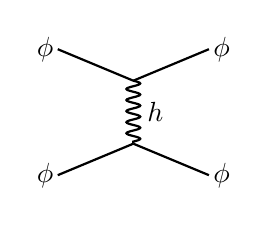
\begin{tikzpicture}[scale=0.8]
  \draw[thick] (-1.2,1)--(0,0.5); \draw[thick] (-1.2,-1)--(0,-0.5);
  \draw[thick] (1.2,1)--(0,0.5);  \draw[thick] (1.2,-1)--(0,-0.5);
  \draw[thick,decorate,decoration={coil,aspect=0,segment length=4pt}] (0,0.5)--(0,-0.5);
  \node at (-1.4,1) {$\phi$}; \node at (-1.4,-1) {$\phi$};
  \node at (1.4,1) {$\phi$};  \node at (1.4,-1) {$\phi$};
  \node at (0.35,0) {$h$};
\end{tikzpicture}
\caption{$t$-channel (plus $s$, $u$)}
\end{subfigure}
\hfill
\begin{subfigure}{0.3\textwidth}
\centering
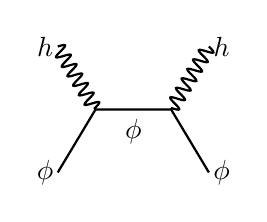
\begin{tikzpicture}[scale=0.8]
  \draw[thick] (-1.2,-1)--(-0.6,0)--(0.6,0)--(1.2,-1);
  \draw[thick,decorate,decoration={coil,aspect=0,segment length=4pt}] (-1.2,1)--(-0.6,0);
  \draw[thick,decorate,decoration={coil,aspect=0,segment length=4pt}] (1.2,1)--(0.6,0);
  \node at (-1.4,1) {$h$}; \node at (1.4,1) {$h$};
  \node at (-1.4,-1) {$\phi$}; \node at (1.4,-1) {$\phi$};
  \node at (0,-0.35) {$\phi$};
\end{tikzpicture}
\caption{Compton, $s$/$u$-channel}
\end{subfigure}
\hfill
\begin{subfigure}{0.3\textwidth}
\centering
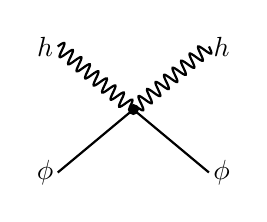
\begin{tikzpicture}[scale=0.8]
  \draw[thick] (-1.2,-1)--(0,0)--(1.2,-1);
  \draw[thick,decorate,decoration={coil,aspect=0,segment length=4pt}] (-1.2,1)--(0,0);
  \draw[thick,decorate,decoration={coil,aspect=0,segment length=4pt}] (1.2,1)--(0,0);
  \fill (0,0) circle (2.5pt);
  \node at (-1.4,1) {$h$}; \node at (1.4,1) {$h$};
  \node at (-1.4,-1) {$\phi$}; \node at (1.4,-1) {$\phi$};
\end{tikzpicture}
\caption{Seagull}
\end{subfigure}

\vspace{0.6cm}

\begin{subfigure}{0.3\textwidth}
\centering
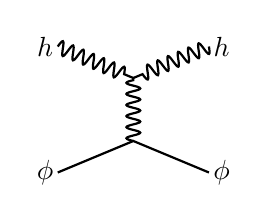
\begin{tikzpicture}[scale=0.8]
  \draw[thick] (-1.2,-1)--(0,-0.5)--(1.2,-1);
  \draw[thick,decorate,decoration={coil,aspect=0,segment length=4pt}] (0,-0.5)--(0,0.5);
  \draw[thick,decorate,decoration={coil,aspect=0,segment length=4pt}] (-1.2,1)--(0,0.5);
  \draw[thick,decorate,decoration={coil,aspect=0,segment length=4pt}] (1.2,1)--(0,0.5);
  \node at (-1.4,1) {$h$}; \node at (1.4,1) {$h$};
  \node at (-1.4,-1) {$\phi$}; \node at (1.4,-1) {$\phi$};
\end{tikzpicture}
\caption{$t$-channel with $hhh$}
\end{subfigure}
\hfill
\begin{subfigure}{0.3\textwidth}
\centering
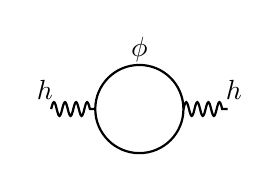
\begin{tikzpicture}[scale=0.8]
  \draw[thick,decorate,decoration={coil,aspect=0,segment length=4pt}] (-1.4,0)--(-0.7,0);
  \draw[thick,decorate,decoration={coil,aspect=0,segment length=4pt}] (0.7,0)--(1.4,0);
  \draw[thick] (0,0) circle (0.7);
  \node at (0,0.95) {$\phi$};
  \node at (-1.5,0.3) {$h$}; \node at (1.5,0.3) {$h$};
\end{tikzpicture}
\caption{$h$ self-energy, $S=1/2$}
\end{subfigure}
\hfill
\begin{subfigure}{0.3\textwidth}
\centering
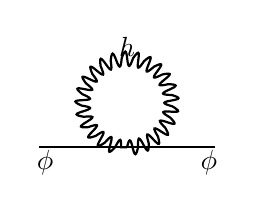
\begin{tikzpicture}[scale=0.8]
  \draw[thick] (-1.4,-0.7)--(1.4,-0.7);
  \draw[thick,decorate,decoration={coil,aspect=0,segment length=4pt}] (0,-0.7) arc (-90:270:0.7);
  \node at (0,0.9) {$h$};
  \node at (-1.3,-0.95) {$\phi$}; \node at (1.3,-0.95) {$\phi$};
\end{tikzpicture}
\caption{$\phi$ self-energy}
\end{subfigure}
\caption{Topologies contributing at $O(\kappa^{2})$. Straight lines: scalar; wavy lines:
graviton. Internal graviton lines require the De Donder propagator, since the TT projector
is a projector on shell only.}
\label{fig:diagrams}
\end{figure}



\subsection{Feynman rules}

\paragraph{Propagators.}
\begin{align}
\text{scalar:}\qquad
\langle 0|T^{*}\phi(x)\phi(y)|0\rangle
&=\int\!\frac{d^4k}{(2\pi)^4}\,
\frac{i\,e^{-ik(x-y)}}{k^{2}-m^{2}+i\epsilon},\\[0.3cm]
\text{graviton (De Donder):}\qquad
\langle 0|T^{*}h_{\mu\nu}(x)h_{\alpha\beta}(y)|0\rangle
&=\int\!\frac{d^4k}{(2\pi)^4}\,
\frac{i\,P^{\rm H}_{\mu\nu,\alpha\beta}}{k^{2}+i\epsilon}\,e^{-ik(x-y)},
\\[0.3cm]
\text{graviton (TT):}\qquad
\langle 0|T^{*}h_{ij}(x)h_{kl}(y)|0\rangle
&=\int\!\frac{d^4k}{(2\pi)^4}\,
\frac{i\,\Lambda^{\rm TT}_{ij,kl}}{k^{2}+i\epsilon}\,e^{-ik(x-y)},
\label{gravprop}
\end{align}
with $P^{\rm H}$ the De Donder projector defined above and $\Lambda^{\rm H}$ the TT 
projector. 

\paragraph{External legs.}
Scalars contribute $1$. External gravitons contribute a TT polarisation tensor
$\varepsilon_{ij}^{(\lambda)}(\hat k)$, $\lambda=+,\times$, satisfying
\begin{equation}
    \epsilon_{ij}=\epsilon_{ji},\qquad
    \delta^{ij}\epsilon_{ij}=0,\qquad
    k^{i}\epsilon_{ij}=0,\qquad
    \epsilon^{(\lambda)}_{ij}\epsilon^{(\lambda')\,ij}=\delta^{\lambda\lambda'},
\end{equation}

\newpage


 
\section{Graviton--Scalar Compton Scattering}
 
We consider the process
\begin{equation}
\varphi(k_3)+h(k_4,\lambda_4)\;\longrightarrow\;\varphi(k_1)+h(k_2,\lambda_2),
\end{equation}
so that the initial and final states are
\begin{equation}
\ket{i}=\ket{k_3;k_4,\lambda_4},
\qquad
\bra{f}=\bra{k_1;k_2,\lambda_2}.
\end{equation}
It is convenient to factor out once and for all
\begin{empheq}[box=\fbox]{equation}
\mathcal{N}\;\equiv\;
\frac{\delta^{(4)}\bigl(k_{\rm in}-k_{\rm out}\bigr)}
{(2\pi)^{2}\sqrt{16\,E_1E_2E_3E_4}},
\label{eq:N}
\end{empheq}
where $E_1,E_3$ are the scalar energies and $E_2=\omega_2$, $E_4=\omega_4$ the graviton
ones. Each contribution of $\hat S$ will be written in the form
\begin{equation}
S_{fi}^{(\alpha)}=i\,\kappa^{2}\,\mathcal{N}\;\mathcal{M}^{(\alpha)}.
\end{equation}
 
There are four topologies at $O(\kappa^2)$: the one-vertex seagull, the $s$- and
$u$-channel scalar exchange, and the $t$-channel graviton exchange mediated by the
cubic graviton self-interaction. We treat them in turn.
 
\subsection{One-vertex contribution: seagull}
 
At first order,
\begin{equation}
S^{\rm sg}_{fi}=-i\int d^{4}x\;
\bra{k_1,k_2\lambda_2}\mathcal{H}_{hh\varphi\varphi}(x)\ket{k_3,k_4\lambda_4}.
\end{equation}
Inserting the mode expansions and retaining the terms that annihilate $k_3,k_4$ and create
$k_1,k_2$, we obtain
\begin{align}
S^{\rm sg}_{fi}=\;&i\kappa^{2}
\int d^{4}x
\int\frac{d^{3}q_1\,d^{3}q_2\,d^{3}q_3\,d^{3}q_4}
{(2\pi)^{6}\sqrt{16E_{q_1}E_{q_2}E_{q_3}E_{q_4}}}
\sum_{\lambda,\lambda'}
e^{i(q_1+q_2-q_3-q_4)x}\notag\\
&\times\Bigl\{
-\tfrac18\,\epsilon_{\alpha\beta}(q_2,\lambda)\epsilon^{\alpha\beta}(q_4,\lambda')
\bigl(q_1\!\cdot\!q_3-m^{2}\bigr)\cdot 4\notag\\
&\qquad
+\tfrac12\,\epsilon^{\mu\alpha}(q_2,\lambda)\,\epsilon^{\nu}{}_{\alpha}(q_4,\lambda')
\bigl(q_{1\mu}q_{3\nu}+q_{3\mu}q_{1\nu}\bigr)\cdot 2
\Bigr\}\notag\\
&\times
\bra{0}\hat a_{k_1}\hat a_{k_2\lambda_2}\,
\hat a^{\dagger}_{q_1}\hat a^{\dagger}_{q_2\lambda}\hat a_{q_3}\hat a_{q_4\lambda'}\,
\hat a^{\dagger}_{k_3}\hat a^{\dagger}_{k_4\lambda_4}\ket{0}.
\label{seagull}
\end{align}
Carrying out the momentum integrals and contractions gives
\begin{empheq}[box=\fbox]{equation}
\mathcal{M}^{\rm sg}=
-\frac{\epsilon^{(2)}\!\cdot\epsilon^{(4)}}{2}\,
\bigl(k_1\!\cdot\!k_3-m^{2}\bigr)
+\epsilon^{(2)*\,\mu\alpha}\,\epsilon^{(4)\,\nu}{}_{\alpha}\,
\bigl(k_{1\mu}k_{3\nu}+k_{3\mu}k_{1\nu}\bigr),
\label{eq:Msg}
\end{empheq}
where $\epsilon^{(2)}\!\cdot\epsilon^{(4)}\equiv
\epsilon^{(2)}_{\alpha\beta}\epsilon^{(4)\alpha\beta}$.
The trace part has been dropped since
all gravitons here are projected into TT gauge $h=0$.
 
\subsection{Two-vertex contribution: virtual scalar exchange}
 
At second order, with two vertices,
\begin{equation}
S^{s+u}_{fi}=-\frac{1}{2}\int d^{4}x_1\,d^{4}x_2\;
\bra{k_1,k_2\lambda_2}
T\bigl\{\mathcal{H}_{h\varphi\varphi}(x_1)\,\mathcal{H}_{h\varphi\varphi}(x_2)\bigr\}
\ket{k_3,k_4\lambda_4},
\end{equation}
the two internal $\varphi$'s are contracted into the Feynman propagator,
\begin{equation}
\c{\varphi(x_1)}\,\c{\varphi(x_2)}=D_F(x_1-x_2).
\end{equation}
Inserting the mode expansions and keeping the terms that annihilate $k_3,k_4$ and create
$k_1,k_2$,
\begin{align}
S^{s}_{fi}=\;&-\kappa^{2}
\int d^{4}x_1\,d^{4}x_2
\int\frac{d^{4}q}{(2\pi)^{4}}
\int\frac{d^{3}q_1\,d^{3}q_2\,d^{3}q_3\,d^{3}q_4}
{(2\pi)^{6}\sqrt{16E_{q_1}E_{q_2}E_{q_3}E_{q_4}}}
\sum_{\lambda,\lambda'}
e^{i(q_1+q_2)x_1}e^{-i(q_3+q_4)x_2}\notag\\
&\times\;\frac{1}{8}\cdot8\;
\frac{e^{-iq(x_1-x_2)}}{q^{2}-m^{2}+i\varepsilon}\;
\Bigl[q^{\mu}q_{1}^{\nu}\,\epsilon_{\mu\nu}(q_2,\lambda)\Bigr]
\Bigl[q^{\rho}q_{3}^{\sigma}\,\epsilon_{\rho\sigma}(q_4,\lambda')\Bigr]\notag\\
&\times
\bra{0}\hat a_{k_1}\hat a_{k_2\lambda_2}\,
\hat a^{\dagger}_{q_1}\hat a^{\dagger}_{q_2\lambda}\hat a_{q_3}\hat a_{q_4\lambda'}\,
\hat a^{\dagger}_{k_3}\hat a^{\dagger}_{k_4\lambda_4}\ket{0},
\label{eq:sfull}
\end{align}
and analogously for $S^u_{fi}$ with $k_2\leftrightarrow k_4$.
The spacetime integrations fix the internal momentum to
\begin{equation}
q=k_3+k_4\quad(s),
\qquad
q=k_3-k_2\quad(u),
\end{equation}
so that
\begin{equation}
q^{2}-m^{2}=2k_3\!\cdot\!k_4=2k_1\!\cdot\!k_2 \quad(s),
\qquad
q^{2}-m^{2}=-2k_3\!\cdot\!k_2\quad(u).
\end{equation}

At each vertex the internal momentum is contracted with a graviton polarization, and
transversality removes it:
\begin{equation}
q^{\nu}\epsilon^{(4)}_{\mu\nu}=(k_3+k_4)^{\nu}\epsilon^{(4)}_{\mu\nu}
=k_3^{\nu}\epsilon^{(4)}_{\mu\nu},
\end{equation}
and likewise at the other vertex. Finally we recover
\begin{empheq}[box=\fbox]{align}
\mathcal{M}^{s}&=
-\frac{1}{2k_1\!\cdot\!k_2+i\varepsilon}\;
\bigl(k_3^{\mu}k_3^{\nu}\epsilon^{(4)}_{\mu\nu}\bigr)
\bigl(k_1^{\rho}k_1^{\sigma}\epsilon^{(2)}_{\rho\sigma}\bigr),\\[1mm]
\mathcal{M}^{u}&=
+\frac{1}{2k_3\!\cdot\!k_2+i\varepsilon}\;
\bigl(k_3^{\mu}k_3^{\nu}\epsilon^{(2)}_{\mu\nu}\bigr)
\bigl(k_1^{\rho}k_1^{\sigma}\epsilon^{(4)}_{\rho\sigma}\bigr).
\label{eq:Msu}
\end{empheq}
The trace term has again been discarded.
 
\subsection{Two-vertex contribution: graviton self-interaction}
 
The last topology is the $t$-channel exchange of an internal graviton: one end attaches
to the scalar line through $\mathcal{H}_{h\varphi\varphi}$, the other to the two external
gravitons through the cubic self-interaction
\begin{equation}
S^{(3)}_{HE} = \int d^4x\, \mathcal{L}_g^1, \qquad
\mathcal{L}_g^1 =\;\kappa  \Bigl[
\underbrace{\tfrac{1}{2} h_\beta^\alpha \partial^\mu h_\alpha^\beta \partial_\mu h}_{(1)}
\underbrace{- \tfrac{1}{2} h_\beta^\alpha \partial_\alpha h_\nu^\mu \partial^\beta h_\mu^\nu}_{(2)}
\underbrace{- h_\beta^\alpha \partial_\mu h_\alpha^\nu \partial^\mu h_\nu^\beta}_{(3)}
+ \underbrace{\tfrac{1}{4} h\, \partial^\beta h_\nu^\mu \partial_\beta h_\mu^\nu}_{(4)}
+ \underbrace{h_\mu^\beta \partial_\nu h_\beta^\alpha \partial^\mu h_\alpha^\nu}_{(5)}
\underbrace{- \tfrac{1}{8} h\, \partial^\nu h\, \partial_\nu h}_{(6)} \Bigr].
\label{eq:Lg1}
\end{equation}
As in the seagull calculation, the pure-trace term (6) does not contribute once the
external gravitons are put in TT gauge, so only terms (1)--(5) survive. Each is
evaluated by attaching to its two internal legs the propagator numerator (de Donder
gauge)
\begin{equation}
P^{\mu\nu,\rho\sigma}=\tfrac12\bigl(\eta^{\mu\rho}\eta^{\nu\sigma}
+\eta^{\mu\sigma}\eta^{\nu\rho}-\eta^{\mu\nu}\eta^{\rho\sigma}\bigr),
\end{equation}
and to its remaining open indices the scalar-line vertex factor $2k_1^\rho k_3^\sigma$,
with the internal momentum fixed by conservation to $q=k_1-k_3=k_4-k_2$. We use the
shorthand
\begin{equation}
a\cdot\epsilon\cdot b\equiv a^\mu\epsilon_{\mu\nu}b^\nu,
\qquad
a\cdot\epsilon\cdot\epsilon'\cdot b\equiv a^\mu\epsilon_{\mu\nu}\epsilon'^{\nu\rho}b_\rho.
\end{equation}
The last line of each block below is the result after taking the classical
(soft-graviton, heavy-scalar) limit, in which $E,\omega$ are the scalar and graviton
energies, $n_2,n_4$ the unit vectors along $\vec k_2,\vec k_4$, and $\upsilon$ the
scalar velocity.
 
\bigskip
\noindent\textbf{Term (1).}
\begin{align*}
\tfrac12 h_\beta^\alpha \partial^\mu h_\alpha^\beta \partial_\mu h
&= \tfrac12\,(\epsilon^{(2)}\!\cdot\epsilon^{(4)})\,\bigl[q\cdot(k_4-k_2)\bigr]\;
\mathrm{Tr}P\,(2k_{1\mu}k_{3\nu}) \\
&= -(\epsilon^{(2)}\!\cdot\epsilon^{(4)})\,(k_1\!\cdot\!k_3)(-2k_2\!\cdot\!k_4) \\
&\overset{\sim}{=}\ 2(E\omega)^2(\epsilon^{(2)}\!\cdot\epsilon^{(4)})(1-n_2\!\cdot\!n_4)
\end{align*}
 
\bigskip
\noindent\textbf{Term (2).}
\begin{align*}
-\tfrac12 h_\beta^\alpha \partial_\alpha h_\nu^\mu \partial^\beta h_\mu^\nu
&= -\tfrac12\Big\{(\epsilon^{(2)}\!\cdot\epsilon^{(4)})\,(2k_{2\alpha}k_{4\beta}P^{\alpha\beta,\mu\nu})(2k_{1\mu}k_{3\nu}) \\
&\qquad +2\big[(k_4\!\cdot\!\epsilon^{(2)}\!\cdot\! q)(\epsilon^{(4)}_{\alpha\beta}P^{\alpha\beta,\mu\nu})(2k_{1\mu}k_{3\nu})-(2\leftrightarrow4)\big]\Big\} \\[4pt]
&= -\tfrac12\Big\{4(\epsilon^{(2)}\!\cdot\epsilon^{(4)})\Big[\tfrac12(k_1\!\cdot\!k_2)(k_3\!\cdot\!k_4)+\tfrac12(k_1\!\cdot\!k_4)(k_3\!\cdot\!k_2)-\tfrac12(k_2\!\cdot\!k_4)(k_1\!\cdot\!k_3)\Big] \\
&\qquad +4\Big[(k_4\!\cdot\!\epsilon^{(2)}\!\cdot\! q)\bigl(k_1\!\cdot\!\epsilon^{(4)}\!\cdot\! k_3-\epsilon^{(4)}\!\cdot\!k_1k_3\bigr)-(k_2\!\cdot\!\epsilon^{(4)}\!\cdot\! q)(k_1\!\cdot\!\epsilon^{(4)}\!\cdot\! k_3)\Big]\Big\} \\[4pt]
&\overset{\sim}{=}\ -\tfrac{(E\omega)^2}{2}\Big\{4(\epsilon^{(2)}\!\cdot\epsilon^{(4)})\Big[\tfrac12(1-n_2\!\cdot\!\upsilon)(1-n_4\!\cdot\!\upsilon)+\tfrac12(1-n_4\!\cdot\!\upsilon)(1-n_2\!\cdot\!\upsilon)-\tfrac12(1-n_2\!\cdot\!n_4)\Big] \\
&\qquad +4\big[(k_4\!\cdot\!\epsilon^{(2)}\!\cdot\! k_4)\,O(\upsilon^2)+O(\upsilon^2)\big]\Big\} \\[4pt]
&\overset{\sim}{=}\ -2(E\omega)^2(\epsilon^{(2)}\!\cdot\epsilon^{(4)})\Big(\tfrac12-n_2\!\cdot\!\upsilon-\upsilon\!\cdot\! n_4+\tfrac{n_2\!\cdot\!n_4}{2}\Big) \\[4pt]
&\overset{\sim}{=}\ -(E\omega)^2(\epsilon^{(2)}\!\cdot\epsilon^{(4)})\bigl[1-2n_2\!\cdot\!\upsilon-2\upsilon\!\cdot\! n_4+n_2\!\cdot\!n_4\bigr]
\end{align*}
 
\bigskip
\noindent\textbf{Term (3).}
\begin{align*}
-h_\beta^\alpha\partial_\mu h_\alpha^\nu\partial^\mu h_\nu^\beta
&= -\Big\{2\,\epsilon^{(2)\,\nu\alpha}\epsilon^{(4)\,\beta}_{\ \ \nu}(k_2\!\cdot\!k_4)\,P_{\alpha\beta}{}^{\rho\sigma}(2k_{1\rho}k_{3\sigma}) \\
&\qquad +\big[\epsilon^{(2)}_{\ \beta}{}^{\alpha}\epsilon^{(4)\,\beta\nu}(k_4\!\cdot\! q)\,P^{\rho\sigma}{}_{\nu\alpha}(2k_{1\rho}k_{3\sigma})-(2\leftrightarrow4)\big] \\
&\qquad +\big[\epsilon^{(2)}_{\ \beta}{}^{\alpha}\epsilon^{(4)}_{\alpha\nu}(k_4\!\cdot\! q)\,P_{\rho\sigma}{}^{\nu\beta}(2k_1{}^\rho k_3{}^\sigma)-(2\leftrightarrow4)\big]\Big\} \\[4pt]
&= -\Big\{4\Big[\tfrac12(k_1\!\cdot\!\epsilon^{(2)}\!\cdot\!\epsilon^{(4)}\!\cdot\! k_3)+\tfrac12(k_3\!\cdot\!\epsilon^{(2)}\!\cdot\!\epsilon^{(4)}\!\cdot\! k_1)-\tfrac12(\epsilon^{(2)}\!\cdot\epsilon^{(4)})(k_1\!\cdot\!k_3)\Big](k_2\!\cdot\!k_4) \\
&\qquad +4\Big[\tfrac12(k_1\!\cdot\!\epsilon^{(2)}\!\cdot\!\epsilon^{(4)}\!\cdot\! k_3)+\tfrac12(k_3\!\cdot\!\epsilon^{(2)}\!\cdot\!\epsilon^{(4)}\!\cdot\! k_1)-\tfrac12(\epsilon^{(2)}\!\cdot\epsilon^{(4)})(k_1\!\cdot\!k_3)\Big](k_4\!\cdot\! q)+\cdots\Big\} \\[4pt]
&\overset{\sim}{=}\ -\Big\{-2(\epsilon^{(2)}\!\cdot\epsilon^{(4)})(1-n_2\!\cdot\!n_4)+2\big[(\epsilon^{(2)}\!\cdot\epsilon^{(4)})(k_2\!\cdot\!k_4)+(\epsilon^{(2)}\!\cdot\epsilon^{(4)})(k_4\!\cdot\!k_2)\big]\Big\} \\[4pt]
&\overset{\sim}{=}\ -2(E\omega)^2(\epsilon^{(2)}\!\cdot\epsilon^{(4)})(1-n_2\!\cdot\!n_4)
\end{align*}
(the omitted terms, denoted $\cdots$, cancel or are subleading in the limit above).
 
\bigskip
\noindent\textbf{Term (4).}
\begin{align*}
\tfrac14 h\,\partial^\beta h_\nu^\mu \partial_\beta h_\mu^\nu
&= \tfrac14\Big\{2(k_2\!\cdot\!k_4)(\epsilon^{(2)}\!\cdot\epsilon^{(4)})(-\eta^{\mu\nu})(2k_{1\mu}k_{3\nu})\Big\} \\
&\overset{\sim}{=}\ -(E\omega)^2(\epsilon^{(2)}\!\cdot\epsilon^{(4)})(1-n_2\!\cdot\!n_4)
\end{align*}
 
\bigskip
\noindent\textbf{Term (5).}
\begin{align*}
h_\mu^\beta\partial_\nu h_\beta^\alpha\partial^\mu h_\alpha^\nu
&= \Big\{\big[k_{2\nu}k_{4\mu}\,\epsilon^{(2)\,\alpha}{}_{\beta}\,\epsilon^{(4)\,\nu}{}_{\alpha}\,P^{\mu\beta}{}_{\rho\sigma}(2k_1{}^\rho k_3{}^\sigma)+(2\leftrightarrow4)\big] \\
&\qquad -\big[\epsilon^{(2)}_{\mu\beta}\epsilon^{(4)\,\nu}{}_{\alpha}\, k_{2\nu}k_4{}^\mu P^{\beta\alpha}{}_{\rho\sigma}+(2\leftrightarrow4)\big](2k_1{}^\rho k_3{}^\sigma) \\
&\qquad +\big[\epsilon^{(2)}_{\mu}{}^\beta\epsilon^{(4)}_{\beta\alpha}k_{4\nu}q^\mu P^{\alpha\mu}{}_{\rho\sigma}-(2\leftrightarrow4)\big](2k_1{}^\rho k_3{}^\sigma)\Big\} \\[4pt]
&= \Big\{(k_4\!\cdot\!k_1)(k_3\!\cdot\!\epsilon^{(2)}\!\cdot\!\epsilon^{(4)}\!\cdot\! k_2)+(k_4\!\cdot\!k_3)(k_1\!\cdot\!\epsilon^{(2)}\!\cdot\!\epsilon^{(4)}\!\cdot\! k_2)-(k_1\!\cdot\!k_3)(k_4\!\cdot\!\epsilon^{(2)}\!\cdot\!\epsilon^{(4)}\!\cdot\! k_2) \\
&\qquad +(k_2\!\cdot\!k_1)(k_3\!\cdot\!\epsilon^{(4)}\!\cdot\!\epsilon^{(2)}\!\cdot\! k_4)+(k_2\!\cdot\!k_3)(k_1\!\cdot\!\epsilon^{(4)}\!\cdot\!\epsilon^{(2)}\!\cdot\! k_4)-(k_1\!\cdot\!k_3)(k_2\!\cdot\!\epsilon^{(4)}\!\cdot\!\epsilon^{(2)}\!\cdot\! k_4) \\
&\qquad +2\big[(k_1\!\cdot\!\epsilon^{(4)}\!\cdot\!\epsilon^{(2)}\!\cdot\! k_4)(k_4\!\cdot\!k_2)+(k_3\!\cdot\!\epsilon^{(2)}\!\cdot\!\epsilon^{(4)}\!\cdot\! k_2)(k_2\!\cdot\!k_1)\big] \\
&\qquad -2\big[(k_1\!\cdot\!\epsilon^{(2)}\!\cdot\! k_4)(k_2\!\cdot\!\epsilon^{(4)}\!\cdot\! k_2)+(k_3\!\cdot\!\epsilon^{(2)}\!\cdot\! k_4)(k_1\!\cdot\!\epsilon^{(4)}\!\cdot\! k_2)-(k_1\!\cdot\!\epsilon^{(2)}\!\cdot\!\epsilon^{(4)}\!\cdot\! k_2)(k_1\!\cdot\!k_3)\big]\Big\} \\[4pt]
&\overset{\sim}{=}\ \Big\{4\,\upsilon\!\cdot\!\epsilon^{(2)}\!\cdot\!\epsilon^{(4)}\!\cdot\! n_2+4\,\upsilon\!\cdot\!\epsilon^{(4)}\!\cdot\!\epsilon^{(2)}\!\cdot\! n_4-2\,n_2\!\cdot\!\epsilon^{(4)}\!\cdot\!\epsilon^{(2)}\!\cdot\! n_4\Big\}\epsilon^{(2)}\!\cdot\!\epsilon^{(4)}\!\cdot\! n_2 \\[4pt]
&\overset{\sim}{=}\ (E\omega)^2\Big\{4\,\upsilon\!\cdot\!\epsilon^{(2)}\!\cdot\!\epsilon^{(4)}\!\cdot\! n_2+4\,\upsilon\!\cdot\!\epsilon^{(4)}\!\cdot\!\epsilon^{(2)}\!\cdot\! n_4\Big\}
\end{align*}

\bigskip
\noindent
Summing terms (1)--(5) and simplifying (the $n_2\!\cdot\!n_4$ pieces cancel exactly)
gives

\begin{empheq}[box=\fbox]{equation}
S _{fi} \overset{\sim}{=}
\frac{2 G^2E}{\pi \omega}\frac{1}{\sin ^2 \theta /2} \delta^{(4)}(K_{tot})\big\{ (\epsilon^{(2)}\cdot
\epsilon^{(4)})-\vec{v}\cdot(\vec{n_2}+\vec{n_4})-2(\vec{n_2}\cdot\epsilon^{(4)}\cdot\epsilon^{(2)}\cdot \vec{v}+\vec{n_4}\cdot\epsilon^{(2)}\cdot\epsilon^{(4)}\cdot \vec{v})
\big\} 
\label{eq:Mt}
\end{empheq}
 
 
\newpage

\section{Scattering Amplitude}

\begin{equation}
    d \sigma = \int |S_{fi}|^2 \frac{V}{T J_{in}} d^3p_3 d^3p_4
\end{equation}

If now we consider that:

\begin{itemize}
    \item In infinite mass scatterings, the 4-momentum conservation simplifies into just Energy conservation (Greiner QED p.170)
    \item Due to this, we can consider the massive particle as an exgternal potential
    \item The incoming flux has can be simplified to: $J = |c-v| \approx 1-|v|$
    \item We used many tricks such as the identity $\delta^2(\omega_4-\omega_2) = \delta(0) \delta(\omega_4-\omega_2)$
\end{itemize}

We get:

\begin{equation}
    d \sigma = \int \frac{1}{1-|v|} (32\pi G)^2 \frac{\delta (\omega_4 - \omega_2)}{16E_1 ... E_4}
    \frac{E^4}{sen^4 \theta/2} |\{...\}|^2 d^3p_4
\end{equation}

\begin{equation}
    \approx (1+|v|)(32\pi G)^2 \frac{E^2}{16} \int d |p_4| d \Omega_4 \delta(|p_4|-|p_2|)\frac{|p_4|}{|p_2|} \frac{|\{...\}|^2}{sen^4 \theta /2}
\end{equation}


\begin{equation}
    \approx (1+|v|)(32\pi G)^2 \frac{E^2}{16} \int d \Omega_4 \frac{|\{...\}|^2}{sen^4 \theta /2}
\end{equation}

\begin{equation}
    \frac{d\sigma}{d \Omega_4} \approx (1+|v|)(32\pi G)^2 \frac{E^2}{16} \frac{|\{...\}|^2}{sen^4 \theta /2}
\end{equation}



Last but not least, we are interested in calculating what's inside the $|\{...\}|^2$ term up to leading order at $v$.

\subsection{Polarization products}
First of all, let's compute the scalar products of the polarization vectors.
We are interested in evaluating the polarization sums appearing in scalar products of polarization vectors. This can be done by explicitly using their geometric construction. The polarization vectors $\epsilon$ live in the transverse plane orthogonal to the spatial momentum and can be expressed as linear combinations of two real orthonormal vectors $u$ and $v$, with
\[
u \cdot v = 0, \qquad u^2 = v^2 = 1.
\]

If we consider two different momenta $k_2$ and $k_4$, we choose the transverse bases such that the plane defined by $k_2$ and $k_4$ is aligned with that defined by $u_2$ and $u_4$. With this choice, the relevant scalar products reduce to
\begin{align}
   u_2 \cdot u_4 &= \cos \theta,\\
   v_2 \cdot v_4 &= 1,\\
   u_2 \cdot v_4 &= v_2 \cdot u_4 = 0.
\end{align}

what we get is:

\begin{align}
    &\epsilon (k_2,+)\cdot \epsilon (k_4, +) = \frac12(cos^2\theta+1)\\
    &\epsilon (k_2,+)\cdot \epsilon (k_4, \times) = 0\\
    &\epsilon (k_2,+)\cdot \epsilon (k_4, +) = cos\, \theta
\end{align}

Finally, from these amplitudes, we can compute the elements $|\epsilon_2 \cdot \epsilon_4|^2$:

\begin{equation}
   \frac{1}{4} \sum_{+,\cross}^{i \;f} |\epsilon_2 \cdot \epsilon_4|^2 = \frac{1+6\cos^2\theta+\cos^4\theta}{8}.
\end{equation}

Further on, the terms $\vec{v}\cdot \vec{n}$ and $(v\epsilon_i\epsilon_j n_i)$ depend on 
the incoming direction of the graviton itself. 
If the incoming graviton is directed like the scattered particle along the $z$ axis, then $\vec{v}\cdot \vec{n_4} = v\cos\theta$ and $\vec{v}\cdot \vec{n_2} = v$. On the other hand
 $(v\epsilon_4\epsilon_2 n_4) = ... $ and $(v\epsilon_2\epsilon_4 n_2)=0$.


 \subsection{Leading order scattering}

 Then, at leading order in velocity, the scattering cross section is:

 \begin{equation}
    \frac{d\sigma}{d\Omega} = 8\pi^2 ( G E)^2 \frac{1+6\cos^2\theta+\cos^4\theta}{ \sin^4 \theta /2})
 \end{equation}
% ====================================================================

\section{Open Quatum Systems}
We will develop the theory of quantum open systems from the point of view of the so-
called Feynman–Vernon influence functional. This approach and its closely
related Schwinger–Keldysh or closed time path method will underlie the anal-
ysis of nonequilibrium quantum fields.

We start from the path integral representation of the unitary evolution operator $U(t)$:

\[
\langle x,t\mid U(t)\mid x_0,0\rangle = \int_{x(0)=x_0}^{x(t)=x} \mathcal{D}x\; e^{\tfrac{i}{\hbar}S[x]}
\]

Since in open quantum systems we are interested in density matrix $\rho$:

\begin{align}
\rho(x,x',t) &= \langle x\,|\,U(t)\,\rho\,U^\dagger(t)\,|\,x'\rangle \\
&= \int_{x(0)=x_i}^{x(t)=x}\mathcal{D}x\int_{x'(0)=x_i'}^{x'(t)=x'}\mathcal{D}x'\;\exp\left\{\frac{i}{\hbar}\big(S[x]-S[x']\big)\right\}\;\rho\big(x_i,x_i',0\big).
\end{align}

Since the hermitian coniugate of the evolution operators evolves the bra and not the ket.
What we have is the evolution of two histories rather than one. 
Equivalently, we could think of a unique path integral, with a forward evolution then a 
backward one. The reason we speak of backward evolution is the sign
of the action, which leds to anti-time ordering of the operators. In path integral QFT,
we recover propagators by integrating over paths two fields. If we do the same 
here what we get is really interesting: defining what field we are integrating, we get
different evolutions.

\begin{align}
G_{11}(\tau,\tau')
&=
\int \mathcal{D}x\,\mathcal{D}x'\,
e^{i\left(S[x]-S[x']\right)}
\,\rho\!\left(x(0),x'(0),0\right)\,
x(\tau)\,x(\tau')
\nonumber\\
&\equiv
\left\langle
\hat X(\tau)\hat X(\tau')
\right\rangle .
\end{align}

The reason is that we can decompose the path integral over times:

\begin{align}
G_{11}(\tau,\tau')
&=
\int dx(0)\,dx'(0)\,dx(\tau')\,dx(\tau)\,dx(t)
\nonumber\\
&\quad\times
\int_{x(0)}^{x(\tau')}
\mathcal{D}x\,
e^{iS[x]}
\;
x(\tau')
\int_{x(\tau')}^{x(\tau)}
\mathcal{D}x\,
e^{iS[x]}
\;
x(\tau)
\nonumber\\
&\quad\times
\int_{x(\tau)}^{x(t)}
\mathcal{D}x\,
e^{iS[x]}
\int_{x'(0)}^{x(t)}
\mathcal{D}x'\,
e^{-iS[x']}
\;
\rho\!\left(x(0),x'(0),0\right).
\end{align}

And from the traces we get the starting results:

\begin{align}
G_{11}(\tau,\tau')
&=
\int dx(0)\,dx'(0)\,dx(\tau')\,dx(\tau)\,dx(t)
\nonumber\\
&\quad\times
\langle x(t)|U(t,\tau)|x(\tau)\rangle\,
x(\tau)\,
\langle x(\tau)|U(\tau,\tau')|x(\tau')\rangle\,
x(\tau')
\nonumber\\
&\quad\times
\langle x(\tau')|U(\tau',0)|x(0)\rangle\,
\langle x(0)|\rho(0)|x'(0)\rangle\,
\langle x'(0)|U(0,t)|x(t)\rangle.
\end{align}

\begin{equation}
G_{11}(\tau,\tau')
=
\operatorname{Tr}
\!\left[
U(t,\tau)\,
\hat X\,
U(\tau,\tau')\,
\hat X\,
U(\tau',0)\,
\rho(0)\,
U(0,t)
\right]\equiv
\left\langle
\hat X(\tau)\hat X(\tau')
\right\rangle .
\end{equation}

For $G^{22}$ we get the same result but with time ordering reversed, since we 
could make the substitution $t\to -t$ to recover a positive action.
On the other hand:

\begin{equation}
G_{12}(\tau,\tau')
=
\int \mathcal{D}x\,\mathcal{D}x'\;
e^{i(S[x]-S[x'])}\,
\rho\!\big(x(0),x'(0),0\big)\,
x(\tau)\,x'(\tau')
\quad \text{con } x(t)=x'(t).
\end{equation}

\begin{equation}
G_{12}(\tau,\tau')
=
\mathrm{Tr}\Big[
U(0,\tau')\,\hat X\,
U(\tau',t)\,U(t,\tau)\,\hat X\,
U(\tau,0)\,\rho(0)
\Big].
\end{equation}

Primed operators, so primed fields, come always on the left. 

\section{Influence Functional}

\subsection{Reduced density matrix and definition of the influence functional}

\[
\begin{aligned}
\rho(x_q,q,t)
&= \langle x_q,q,t|\rho|x'_q,q,t\rangle \\
&= \int dx_i\,dq_i\,dx'_i\,dq'_i\;
\langle x_q,q,t|x_i,q_i,0\rangle\,
\langle x_i,q_i,0|\rho|x'_i,q'_i,0\rangle\,
\langle x'_i,q'_i,0|x'_q,q,t\rangle \\
&= \int dx_i\,dq_i\,dx'_i\,dq'_i\;
\left(\int_{x_i,q_i}^{x_q,q}\mathcal{D}x\,\mathcal{D}q\; e^{iS[x,q]}\right)
\rho(x_i,q_i,x'_i,q'_i,0)
\left(\int_{x'_i,q'_i}^{x'_q,q}\mathcal{D}x'\,\mathcal{D}q'\; e^{-iS[x',q']}\right) \\
&\equiv \int dx_i\,dq_i\,dx'_i\,dq'_i\;
\mathcal{J}(xq,x'q,\,t\,|\,x_iq_i,x'_iq'_i,0)\,
\rho(x_i,q_i,x'_i,q'_i,0)
\end{aligned}
\]

\[
\rho_r(x,x',t)
= \int_{-\infty}^{+\infty} dq\;\rho(x,q,x',q,t).
\]

\[
\rho(x_i,q_i,x'_i,q'_i,0)
=
\rho_S(x_i,x'_i,0)\,\rho_E(q_i,q'_i,0)
\quad\Rightarrow\quad
\rho_r(x,x',t)
=
\int dx_i\,dx'_i\;
J_r(x,x',t|x_i,x'_i,0)\;
\rho_S(x_i,x'_i,0).
\]

\[
J_r(x,x',t|x_i,x'_i,0)
=
\int_{x_i}^{x}\mathcal{D}x
\int_{x'_i}^{x'}\mathcal{D}x'\;
\exp\!\big(iS[x]-iS[x']\big)\;
F[x,x'].
\]

\[
F[x,x'] = \exp\!\big(iS_{\mathrm{IF}}[x,x']\big),
\qquad
F[x,x']
=
\int dq_i\,dq'_i\,dq\;
\rho_E(q_i,q'_i,0)\;
\int_{q_i}^{q}\mathcal{D}q\;
e^{\,i(S_E[q]+S_{\mathrm{int}}[x,q])}
\int_{q'_i}^{q}\mathcal{D}q'\;
e^{-i(S_E[q']+S_{\mathrm{int}}[x',q'])}.
\]

\subsection{General properties of the influence action}

\[
e^{i S_{\mathrm{IF}}[x,x',t]} = \mathrm{Tr}\left\{U_{x'}(0,t)\,U_x(t,0)\,\rho_E(0)\right\}.
\]

\[
S_{\mathrm{IF}}[x,x,t]=0,
\qquad
S_{\mathrm{IF}}[x',x,t] = - S_{\mathrm{IF}}^*[x,x',t].
\]

\[
u(t)=x(t)-x'(t), \qquad X(t)=\frac{x(t)+x'(t)}{2},
\]
\[
S_{\mathrm{IF}}[X,u,t]
=
\sum_{k=1}^{\infty}
\frac{1}{k!}
\int dt_1 \cdots dt_k\,
S^{(k)}[X;t_1,\dots,t_k;t]\,
u(t_1)\cdots u(t_k),
\]
odd orders real, even orders imaginary.

\[
\left.\frac{\delta S_{\mathrm{IF}}}{\delta x}\right|_{x=x'}
=
-
\left.\frac{\delta S_{\mathrm{IF}}}{\delta x'}\right|_{x=x'}.
\]

CTP doublet:
\[
x^a(t), \quad a=1,2, \quad x^1=x,\ x^2=x',
\qquad
c_{ab}=\mathrm{diag}(1,-1), \quad c^{ab}=\mathrm{diag}(1,-1),
\]
\[
\int dt\, c_{ab}\,\dot{x}^a \dot{x}^b
=
\int dt\left(\dot{x}^2-\dot{x}'^2\right),
\qquad
S[x^a] = S[x]-S[x'].
\]

\subsection{Application to linearized gravity: the graviton as environment}

System: $\phi$. Environment: $h_{ij}$.

\subsubsection{Graviton action}

\[
S_{HE}^{(2)} = -\frac12\int d^4x\,d^4x'\; h^{ij}(x)\,L_{ij}^{kl}(x,x')\,h_{kl}(x'),
\qquad
L_{ij}^{kl} = \frac{1}{\kappa^2}\,\delta^{(4)}(x-x')\,\eta_i^k\eta_j^l\,\Box.
\]

\[
S_I^{(1)} = \int d^4x\; h^{ij}B_{ij}, \qquad B_{ij} = -\tfrac12\partial_i\phi\,\partial_j\phi.
\]

There is also $S_I^{(2)}=-\frac12\int h\,C\,h$, but at leading order $M=L+C\approx L$: $C$ is dropped from here on.

\[
F[x,x']
=
e^{iS_{\mathrm{IF}}[\phi,\phi']}
=
\int dh\;dh_i\;dh'_i\;
\rho_E(h_i,h'_i,0)\;
e^{-iA[T\langle hh\rangle,\phi]}\,
e^{-iA'[T\langle h'h'\rangle,\phi']}
\sim e^{-\frac12\int d^4x\; h^{ij}C_{ij}^{kl} h_{kl}}.
\]
Here $h_i,h'_i$ still denote the two copies of the environmental path integral prior to integrating out the initial state — temporary use of the prime, distinct from the convention adopted below. Switch to the CTP formalism (Calzetta): the influence action is the functional Fourier transform of a Gaussian functional of the bath histories, hence remains Gaussian.

\subsubsection{General Gaussian result for a linear coupling}

\textbf{Convention}: from here on $h_{ij}$ and $Q$ are never primed — they are the same operator in the Heisenberg picture, and the CTP branch is encoded in the ordering of the product ($T$, $\bar T$, Wightman), not in a second field. The prime (or $\pm$, cl/$\Delta$) is reserved for system variables: $x,x',\phi,\phi',B,B'$.

\[
S_{\mathrm{IF}}[x_a]
= \frac{1}{2}\int dt\,dt'\, x_a(t)\, M_{ab}(t,t')\, x_b(t').
\]
\[
M_{ab}(t,t')
= -i \left.
\frac{\delta^2}{\delta x_a(t)\,\delta x_b(t')}
e^{i S_{\mathrm{IF}}[x_a]}
\right|_{x_a=0},
\]
\[
\left.
\frac{\delta^2}{\delta x_a(t)\,\delta x_b(t')}
e^{i S_{\mathrm{IF}}[x_a]}
\right|_{x_a=0}
=
-\frac{1}{2}
\int \mathcal{D}q\;
e^{i S_E[q]}
\, Q_a(t)\, Q_b(t')\,
\rho_E(q_1(0),q_2(0),0),
\qquad q_1(T)=q_2(T).
\]
\[
M_{ab}(t,t') =
\begin{pmatrix}
\langle T\, [Q(t)Q(t')]\rangle
& -\,\langle [Q(t')Q(t)]\rangle \\[6pt]
-\,\langle [Q(t)Q(t')]\rangle
& \langle \tilde{T}\, [Q(t)Q(t')]\rangle
\end{pmatrix}.
\]

\[
\frac{i}{2} S_{\mathrm{IF}}
=
\frac{i}{2}\int dt\,dt'\,
\Big[
\langle T Q(t)Q(t')\rangle\, x(t)x(t')
- \langle Q(t')Q(t)\rangle\, x(t)x'(t')
- \langle Q(t)Q(t')\rangle\, x'(t)x(t')
+ \langle \tilde{T} Q(t)Q(t')\rangle\, x'(t)x'(t')
\Big].
\]

With $x = X + u/2$, $x' = X - u/2$:
\[
S_{\mathrm{IF}}
=
\int dt\,dt'\,
u(t)\, D(t,t')\, X(t')
+
\frac{i}{2}\int dt\,dt'\,
u(t)\, N(t,t')\, u(t'),
\]
\[
D(t,t')
=
i\,\theta(t-t')\,\langle [Q(t),Q(t')]\rangle,
\qquad
N(t,t')
=
\frac{1}{2}\,\langle \{Q(t),Q(t')\}\rangle.
\]

\subsubsection{Graviton propagator}

\[
(L^{-1})_{ij}^{kl} = -i\kappa^2\,\delta^{(4)}(x-x')\,\eta_i^k\eta_j^l\,\Box^{-1}
\;\;\Longrightarrow\;\;
\langle 0|T\{h_{ij}(x)h^{kl}(x')\}|0\rangle = i(L^{-1})_{ij}^{kl} = \kappa^2\,\eta_i^k\eta_j^l\,\Box^{-1}\delta^{(4)}(x-x').
\]

\subsubsection{Applying the general result to $h$ and $B_{ij}(\phi)$}

\begin{align}
M^{ijkl}_{ab}(t,t') &= i\Big[
\langle T[h^{ij}(t)h^{kl}(t')]\rangle
-\langle h^{kl}(t')h^{ij}(t)\rangle
-\langle h^{ij}(t)h^{kl}(t')\rangle
+\langle \bar T[h^{ij}(t)h^{kl}(t')]\rangle
\Big]\\
S_{\mathrm{IF}} &= \frac{i}{2}\int dt\,dt'\Big[
\langle T[h^{ij}(t)h^{kl}(t')]\rangle\, B_{ij}(t)B_{kl}(t')
-\langle h^{kl}(t')h^{ij}(t)\rangle\, B_{ij}(t)B'_{kl}(t')\\
& \qquad -\langle h^{ij}(t)h^{kl}(t')\rangle\, B'_{ij}(t)B_{kl}(t')
+\langle \bar T[h^{ij}(t)h^{kl}(t')]\rangle\, B'_{ij}(t)B'_{kl}(t')
\Big].
\end{align}

Note: $h$ is never primed; the system branch is carried only by $B,B'$.

\subsubsection{Classical and difference variables}

With $\phi_\pm=\phi_{\rm cl}\pm\phi_\Delta/2$, $B^\pm_{ij}=-\tfrac12\partial_i\phi_\pm\partial_j\phi_\pm$:
\[
X_B^{ij} = -\frac12\partial^i\phi_{\rm cl}\partial^j\phi_{\rm cl} - \frac18\partial^i\phi_\Delta\partial^j\phi_\Delta, \qquad
u_B^{ij} = -\Big(\partial^i\phi_{\rm cl}\partial^j\phi_\Delta+\partial^i\phi_\Delta\partial^j\phi_{\rm cl}\Big).
\]

\[
S_{\mathrm{IF}}
=\int dt\,dt'\;u_B^{ij}(t)\,D_{ijkl}(t,t')\,X_B^{kl}(t')
+\frac{i}{2}\int dt\,dt'\;u_B^{ij}(t)\,N_{ijkl}(t,t')\,u_B^{kl}(t'),
\]
\[
D_{ijkl}(t,t')=i\,\theta(t-t')\,\langle[h_{ij}(t),h_{kl}(t')]\rangle,\qquad
N_{ijkl}(t,t')=\tfrac12\langle\{h_{ij}(t),h_{kl}(t')\}\rangle.
\]

\newpage
\appendix

\section{Appendix A: from the density matrix to the CTP path integral}

Basis-independent form:
\begin{equation}
F[x,x']
=
\mathrm{Tr}
\!\left[
U(x;t)\,\rho_E(0)\,U^\dagger(x';t)
\right]
=
\int dq\,dq_i\,dq_i'\;
\rho_E(q_i,q_i';0)\;
\langle q|U(x;t)|q_i\rangle\;
\langle q|U^\dagger(x';t)|q_i'\rangle.
\end{equation}

Forward and conjugate amplitudes:
\[
\langle q|U(x;t)|q_i\rangle
=
\int_{q_i}^{q}\mathcal{D}q_+\;
e^{\,i\left(S_E[q_+] + S_{\mathrm{int}}[x,q_+]\right)},
\qquad
\langle q|U^\dagger(x';t)|q_i'\rangle
=
\int_{q_i'}^{q}\mathcal{D}q_-\;
e^{-i\left(S_E[q_-] + S_{\mathrm{int}}[x',q_-]\right)}.
\]
The minus sign in the exponent is not a different dynamics: it comes from complex conjugation of the amplitude. The two integrations combine into a single path integral over the contour $\mathcal C=\mathcal C_+\cup\mathcal C_-$ (forward then backward in time, glued at $t_f$), with free endpoints $q_i,q_i'$ weighted by $\rho_E$:
\begin{equation}
F[x,x']
=
\int dq_i\,dq_i'\;
\rho_E(q_i,q_i';0)
\int_{\mathcal{C}}\mathcal{D}q\;
e^{\,iS_{\mathcal{C}}[q;x,x']},
\qquad
S_{\mathcal{C}} = S_E[q_+]+S_{\rm int}[x,q_+] - \big(S_E[q_-]+S_{\rm int}[x',q_-]\big).
\end{equation}
The only physical difference between the two branches is the operator time ordering.

\section{Appendix B: Gaussian environment and the CTP matrix structure}

\subsection*{Origin of the matrix structure}

The environment field is doubled, $q\to(q_+,q_-)$, $J\to(J_+,J_-)$, contour metric $C=\mathrm{diag}(1,-1)$: a direct consequence of $S[q_+]-S[q_-]$, not an extra assumption.

\subsection*{Gaussian integral, one-component case}

\begin{equation}
Z[J] = \int dq\;\exp\!\left[\frac{i}{2}qKq + iJq\right]
= \mathcal N \exp\!\left[-\frac{i}{2}JK^{-1}J\right].
\end{equation}

\subsection*{CTP case}

\begin{equation}
S[q_+]-S[q_-] = \tfrac12\,q_a K_{ab} q_b, \qquad
K_{ab}(x,x') = \delta^{(4)}(x-x')\,\mathrm{diag}(K,-K).
\end{equation}
$K_{ab}$ is diagonal, but $G_{ab}=(K_{ab})^{-1}$ is not: inverting it is a differential problem that requires boundary conditions (continuity at $t_{\max}$, correlations at $t_i$ fixed by $\rho$), which generate the off-diagonal, state-dependent components:
\begin{equation}
G_{ab} =
\begin{pmatrix}
\langle T[q(x)q(x')]\rangle & \langle q(x')q(x)\rangle \\
\langle q(x)q(x')\rangle & \langle \bar T[q(x)q(x')]\rangle
\end{pmatrix}
= \begin{pmatrix} G_F & G^< \\ G^> & G_{\bar F}\end{pmatrix}.
\end{equation}

\subsection*{Influence functional for a Gaussian environment}

Quadratic environment action, Gaussian $\rho_e$, bilinear coupling $S_{\rm int}=\int dt\,x_a(t)\,Q_a[q(t)]$ with $Q_a$ linear in $q$. The functional Fourier transform of a Gaussian is Gaussian, so $S_{IF}$ is quadratic in $x_+,x_-$:
\begin{equation}
S_{IF} = \frac12\int dt\,dt'\;x_a(t)\,M_{ab}(t,t')\,x_b(t'),
\qquad
M_{ab}(t,t') = -i\,\frac{\delta^2}{\delta x_a(t)\,\delta x_b(t')}\,e^{iS_{IF}[x_a]}\Big|_{x_a=0}.
\end{equation}
Direct variation gives a CTP expectation value of $Q$ with the system-environment coupling switched off, i.e.\ exactly $G_{ab}$ above, evaluated on $Q$ and traced with $\rho_e$:
\begin{equation}
M_{ab}(t,t') = i\,G_{ab}^Q(t,t') = i
\begin{pmatrix}
\langle T[Q(t)Q(t')]\rangle & -\langle Q(t')Q(t)\rangle \\
-\langle Q(t)Q(t')\rangle & -\langle \bar T[Q(t)Q(t')]\rangle
\end{pmatrix}.
\end{equation}
Explicitly, with $x_\pm\equiv x_\pm(t)$, $x_\pm'\equiv x_\pm(t')$:
\begin{equation}
S_{IF} = \frac{i}{2}\int dt\,dt'\Big[
\langle T[Q(t)Q(t')]\rangle\,x_+x_+'
-\langle Q(t')Q(t)\rangle\,x_+x_-'
-\langle Q(t)Q(t')\rangle\,x_-x_+'
+\langle \bar T[Q(t)Q(t')]\rangle\,x_-x_-'
\Big].
\end{equation}
The averages are taken with $Q(t)$ evolving under the free environment Hamiltonian, decoupled from the system — together with Gaussianity of $\rho_e$, this is what keeps $M_{ab}$ closed-form.

\subsection*{Rotation to dissipation and noise}

Keldysh basis $X=(x_++x_-)/2$, $u=x_+-x_-$:
\begin{equation}
S_{IF} = \int dt\,dt'\;\Big[u(t)\,D(t,t')\,X(t') + \frac{i}{2}\,u(t)\,N(t,t')\,u(t')\Big],
\end{equation}
\begin{equation}
D(t,t') = i\,\theta(t-t')\,\big\langle[Q(t),Q(t')]\big\rangle,
\qquad
N(t,t') = \frac12\,\big\langle\{Q(t),Q(t')\}\big\rangle.
\end{equation}

\section{Full linearized theory}
% ====================================================================

Expanding the Einstein–Hilbert action around a flat background generates an infinite 
series of nonlinear self–interaction terms for the gravitational field. At linear order, 
the equations of motion take the form


\[
\mathcal{E}_{\mu\nu}^{\alpha\beta} h_{\alpha\beta}
= \frac{\kappa}{2} T_{\mu\nu},
\]


where \(\mathcal{E}_{\mu\nu}^{\alpha\beta}\) denotes the linearized Einstein operator.

With the allowed gauges, matter fields satisfy


\[
\partial^\mu T_{\mu\nu} = 0,
\]
However, expanding higher orders in \(\kappa\), the gravitational field contributes to its own source. 
The equations of motion can be written schematically as
\begin{equation}
\mathcal{E}_{\mu\nu}^{\alpha\beta} h_{\alpha\beta}
= \frac{\kappa}{2}\left( T_{\mu\nu} + t_{\mu\nu}[h] \right),
\end{equation}
where \(t_{\mu\nu}[h]\) is the energy–momentum pseudotensor arising from the nonlinearities of the Einstein–Hilbert action. 
It is object constructed order by order.

In particular, the contribution at order \(i\) in the expansion is sourced by the term 
\(S^{(i+1)}[h]\) in the action. For example,
\begin{equation}
t_{\mu\nu}^{(2)} \sim \frac{\delta S^{(3)}[h]}{\delta h^{\mu\nu}}.
\end{equation}

This structure shows that the graviton couples to its own effective stress–energy, 
leading to a nonlinear “bootstrap” mechanism: iterating the cubic and higher–order 
vertices reconstructs the full Einstein theory.

Gauge invariance at linear order is expressed by the infinitesimal diffeomorphism
\begin{equation}
\delta_\xi^{(0)} h_{\mu\nu}
= \partial_\mu \xi_\nu + \partial_\nu \xi_\mu,
\end{equation}
while at nonlinear order the full transformation must include terms like $\sim h \partial \xi$, which is the complete expansion of the diffeomorfism.

In summary, the self–interaction structure of the graviton encodes the nonlinear 
completion of the theory, and general covariance emerges as the perturbative 
realization of full diffeomorphism invariance order by order in \(\kappa\).


\section{Discarded Calculus: TT Projector self int}
The contribute from this interaction will be in the form:

\[ 
\mathcal M_{hhh}=\left(k_1^\mu k_3^\nu+k_1^\nu k_3^\mu-\eta^{\mu\nu}(k_1 \cdot k_3-m^2)\right)\frac{\Lambda_{\mu\nu,\alpha\beta}(q)}{q^2+i\epsilon}V^{\alpha\beta}(k_2,\epsilon^{(2)};k_4,\epsilon^{(4)})
\]

It's easier to project the left term with the TT projector, which actually has only spatial components ($\alpha\beta=1,2,3$).
\begin{align}
    \Bigl(k_1^\mu k_3^\nu + k_1^\nu  k_3^\mu-\eta^{\mu\nu}&(k_1 \cdot k_3-m^2)\Bigr)\frac{\Lambda_{\mu\nu}^{\;\;\alpha\beta}}{q^2+i\epsilon} = \\&
    \frac{1}{q^2+i\epsilon}\Bigl[
        k_1^\alpha k_3^\beta +k_1^\beta k_3^\alpha - (\vec{k_1}\cdot \vec{k_3})(\hat{q}_\alpha\hat{q}_\beta-\delta_{\alpha\beta})\\& -(\vec{k_3}\cdot \hat{q})(k_1^\alpha q^\beta+k_1^\beta q^\alpha)) - (\vec{k_1}\cdot \hat{q})(k_3^\alpha q^\beta+k_3^\beta q^\alpha)\\&
        +(\vec{k_1}\cdot\hat{q})(\vec{k_3}\cdot\hat{q})\;\bigl(\delta^{\alpha\beta}+q^\alpha q^\beta\bigr) \;
    \Bigr]
\end{align}\\
At this point, we only have to consider all of Wick contractions with $V^{\alpha\beta}$, the Vortex is:
\begin{align}
\text{Vortex} \; = \;h_{\rho}{}^{\sigma}(x_2)
\Bigg[
\frac12
\partial_{\sigma}h_{\nu}{}^{\mu}(x_2)
\partial^{\rho}h_{\mu}{}^{\nu}(x_2)
+
\partial_{\mu}h_{\sigma}{}^{\nu}(x_2)
\partial^{\mu}h_{\nu}{}^{\rho}(x_2)
-
\partial_{\nu}h_{\sigma}{}^{\alpha}(x_2)
\partial^{\rho}h_{\alpha}{}^{\nu}(x_2)
\Bigg]
\end{align}

For simplicity, we will decompose into 3 contributes depending on wheter we are contracting the first, second or third term:
$V= \mathcal{A}^{(1)}+\mathcal{A}^{(2)}+\mathcal{A}^{(3)}$. What happens is we free the vertex of a term, which will form the propagator, and express everything in terms of the indexed $\mu\nu$. Then, we will pose the on-shell conditions on the free legs:


\begin{align}
\mathcal{A}^{(1)\alpha\beta}
&=
-(k_2)^\beta (k_4)^\alpha\,(\epsilon_2\!\cdot\!\epsilon_4)
-2(k_2\!\cdot\!k_4)\,(\epsilon_2\!\cdot\!\epsilon_4)^{\beta\alpha}
\nonumber\\
&\quad
+(k_4)^\alpha\,(\epsilon_2\!\cdot\!\epsilon_4\!\cdot\!k_2)^\beta
+(k_2)^\alpha\,(\epsilon_4\!\cdot\!\epsilon_2\!\cdot\!k_4)^\beta
\\[1ex]
\mathcal{A}^{(2)\alpha\beta}
&=
-\frac12
(k_4\!\cdot\!\epsilon_2\!\cdot\!q)\,
\epsilon_4^{\alpha\beta}
-\frac12
(k_2\!\cdot\!\epsilon_4\!\cdot\!q)\,
\epsilon_2^{\alpha\beta}
\nonumber\\
&\quad
-(\epsilon_2\!\cdot\!\epsilon_4)^{\alpha\beta}\,
q\!\cdot\!(k_2+k_4)
+(\epsilon_2\!\cdot\!k_4)^\alpha
(\epsilon_4\!\cdot\!q)^\beta
+(\epsilon_4\!\cdot\!k_2)^\alpha
(\epsilon_2\!\cdot\!q)^\beta ,
\\[1ex]
\mathcal{A}^{(3)\alpha\beta}
&=
-\frac12
(q\!\cdot\!\epsilon_2\!\cdot\!k_4)\,
\epsilon_4^{\alpha\beta}
-\frac12
(q\!\cdot\!\epsilon_4\!\cdot\!k_2)\,
\epsilon_2^{\alpha\beta}
\nonumber\\
&\quad
-(\epsilon_2\!\cdot\!\epsilon_4)^{\alpha\beta}
(q\!\cdot\!k_4)
-(\epsilon_4\!\cdot\!\epsilon_2)^{\alpha\beta}
(q\!\cdot\!k_2)
\nonumber\\
&\quad
+(\epsilon_4\!\cdot\!\epsilon_2\!\cdot\!q)^\alpha
k_4^\beta
+(\epsilon_2\!\cdot\!\epsilon_4\!\cdot\!q)^\alpha
k_2^\beta .
\end{align}
Summing all up:


\begin{align}
\mathcal{A}^{(1)\alpha\beta}
&=
-(k_2)^\beta (k_4)^\alpha\,(\epsilon_2\!\cdot\!\epsilon_4)
-2(k_2\!\cdot\!k_4)\,(\epsilon_2\!\cdot\!\epsilon_4)^{\beta\alpha}
\nonumber\\
&\quad
+(k_4)^\alpha\,(\epsilon_2\!\cdot\!\epsilon_4\!\cdot\!k_2)^\beta
+(k_2)^\alpha\,(\epsilon_4\!\cdot\!\epsilon_2\!\cdot\!k_4)^\beta
\\[1ex]
\mathcal{A}^{(2)\alpha\beta}
&=
-
(k_4\!\cdot\!\epsilon_2\!\cdot\!q)\,
\epsilon_4^{\alpha\beta}
-
(k_2\!\cdot\!\epsilon_4\!\cdot\!q)\,
\epsilon_2^{\alpha\beta}
\\[1ex]
\mathcal{A}^{(3)\alpha\beta}
&=
+(\epsilon_4\!\cdot\!\epsilon_2\!\cdot\!q)^\alpha
k_4^\beta
+(\epsilon_2\!\cdot\!\epsilon_4\!\cdot\!q)^\alpha
k_2^\beta .
\end{align}

\section{Discarded compute: Bessel proj}



\subsection{The expanded projector}
\newcommand{\bm}[1]{\boldsymbol{#1}}

We will calculate the propagator in cutoff regime.
Looking at the projector, expanding the product gives a sum of terms organized by degree in $\hat n$:

\begin{align}
2\,\Lambda_{ij,kl}(\hat{\bm n}) = &
\underbrace{\big(\delta_{ik}\delta_{jl}+\delta_{il}\delta_{jk}-\delta_{ij}\delta_{kl}\big)}_{\text{degree }0}
\;-\;\\&
\underbrace{\big(\delta_{ik}\hat n_j\hat n_l+\delta_{jl}\hat n_i\hat n_k+\delta_{il}\hat n_j\hat n_k+\delta_{jk}\hat n_i\hat n_l-\delta_{ij}\hat n_k\hat n_l-\delta_{kl}\hat n_i\hat n_j\big)}_{\text{degree }2}
\;+\;\\&
\underbrace{\hat n_i\hat n_j\hat n_k\hat n_l}_{\text{degree }4}.
\end{align}

The crucial point: the angular integral we will need,
\begin{equation}
I_{ij,kl}(\bm r,k) \equiv \int d\Omega_{\hat n}\;\Lambda_{ij,kl}(\hat{\bm n})\, e^{ik\hat{\bm n}\cdot\bm r},
\end{equation}
reduces, by linearity, to just \emph{three} basic integrals:
\begin{equation}
J^{(0)} \equiv \int d\Omega\; e^{ik\hat{\bm n}\cdot\bm r}, \qquad
J^{(2)}_{ab} \equiv \int d\Omega\; \hat n_a\hat n_b\, e^{ik\hat{\bm n}\cdot\bm r}, \qquad
J^{(4)}_{abcd} \equiv \int d\Omega\; \hat n_a\hat n_b\hat n_c\hat n_d\, e^{ik\hat{\bm n}\cdot\bm r},
\end{equation}
contracted with the $\delta$'s appearing in $\Lambda_{ij,kl}$.

$\hat{\bm n}$ appears in the integrand \emph{only}
through the phase $e^{ik\hat{\bm n}\cdot\bm r}$, and
\begin{equation}
\partial_{r_a}\, e^{ik\hat{\bm n}\cdot\bm r} = ik\,\hat n_a\, e^{ik\hat{\bm n}\cdot\bm r}
\quad\Longrightarrow\quad
\hat n_a\, e^{ik\hat{\bm n}\cdot\bm r} = \frac{1}{ik}\,\partial_{r_a}\, e^{ik\hat{\bm n}\cdot\bm r}.
\end{equation}

Since $\bm r\in\mathbb R^3$ and $\hat{\bm n}\in S^2$ are independent variables,
and the domain $S^2$ does not depend on $\bm r$, the derivative $\partial_{r_a}$
can be freely moved in or out of the integral sign:
\begin{equation}
\int d\Omega\;\hat n_a\, e^{ik\hat{\bm n}\cdot\bm r}
= \frac{1}{ik}\,\partial_{r_a}\int d\Omega\; e^{ik\hat{\bm n}\cdot\bm r}
= \frac{1}{ik}\,\partial_{r_a} J^{(0)}.
\end{equation}
Iterating the procedure $2s$ times:
\begin{equation}
\boxed{\;
\int d\Omega\;\hat n_{a_1}\cdots\hat n_{a_{2s}}\, e^{ik\hat{\bm n}\cdot\bm r}
= \frac{1}{(ik)^{2s}}\,\partial_{a_1}\!\cdots\partial_{a_{2s}}\, J^{(0)}(\bm r,k)
\;}
\end{equation}
where all dependence on $\hat{\bm n}$ has now been transferred onto derivatives
with respect to $\bm r$ of a single scalar function, the zeroth-degree integral:
\begin{equation}
J^{(0)}(\bm r,k) = \int d\Omega\; e^{ik\hat{\bm n}\cdot\bm r} = 4\pi\,\frac{\sin(kr)}{kr} = 4\pi\, j_0(kr), \qquad r=|\bm r|, \quad x=kr,
\end{equation}
We can simplify a lot our calculations 
by noticing that we actually have the zeroth order Bessel function.
Since we are interested
in its derivatives with respect to $r$, we will make
the change of variable $x\equiv kr$.

\subsection{Derivatives of the radial function}

For a function depending on $\bm r$ only through $r=|\bm r|$, i.e.
$G(\bm r)=G(r)$, the following basic geometric identities hold:
\begin{equation}
\partial_a r = \hat r_a, \qquad
\partial_a \hat r_b = \frac{1}{r}\big(\delta_{ab}-\hat r_a\hat r_b\big),
\end{equation}
from which $\partial_a G(r) = G'(r)\,\hat r_a$. For the
 derivatives of increasing order, each is expressible as a combination of
$\delta_{ab}$ and $\hat r_a$ with scalar coefficients built from
$G,G',G'',\dots$ and powers of $1/r$:
\begin{align}
\partial_a\partial_b\, G &= B\,\delta_{ab} + (A-B)\,\hat r_a\hat r_b,
&& A=G'', \quad B=\frac{G'}{r}, \\[4pt]
\partial_a\partial_b\partial_c\partial_d\, G &=
\mathcal P\,T^{(1)}_{abcd} + \mathcal Q\,T^{(2)}_{abcd} + \mathcal R\,T^{(3)}_{abcd},
\end{align}
where
\begin{align}
T^{(1)}_{abcd} &= \delta_{ab}\delta_{cd}+\delta_{ac}\delta_{bd}+\delta_{ad}\delta_{bc}, \\
T^{(2)}_{abcd} &= \delta_{ab}\hat r_c\hat r_d+\delta_{ac}\hat r_b\hat r_d+\delta_{ad}\hat r_b\hat r_c
+\delta_{bc}\hat r_a\hat r_d+\delta_{bd}\hat r_a\hat r_c+\delta_{cd}\hat r_a\hat r_b, \\
T^{(3)}_{abcd} &= \hat r_a\hat r_b\hat r_c\hat r_d,
\end{align}
With coefficients:
\begin{equation}
\mathcal P = \frac{G''}{r^2}-\frac{G'}{r^3}, \qquad
\mathcal Q = \frac{G'''}{r}-\frac{3G''}{r^2}+\frac{3G'}{r^3}, \qquad
\mathcal R = G''''-\frac{6G'''}{r}+\frac{15G''}{r^2}-\frac{15G'}{r^3}.
\end{equation}

\subsection{Substituting $G=j_0(kr)$}

Setting $G(r)=j_0(kr)$, $x\equiv kr$, we can use Spherical Bessel properties (https://dlmf.nist.gov/10.51):

\[j'_n(x) = j_{n-1}(x) - \frac{n+1}{x} j_n(x)
\]
\[
j'_n(x) = \frac{n}{x} j_n(x) - j_{n+1}(x)
\]

all derivatives $G',G'',G''',G''''$ can be written in terms of $j_0(x),j_1(x)$,
\subsection{Explicit Bessel-function form of the derivatives}

We now make Step 3 fully explicit, computing $G',G'',G''',G''''$ for
$G(r)=j_0(kr)$ and plugging them into the coefficients $A,B$ and
$\mathcal P,\mathcal Q,\mathcal R$ derived in Section 5.3.

\paragraph{Successive derivatives.}
With $x\equiv kr$ and using only the two recursions
each derivative with respect to $r$ brings down a factor of $k$ (since
$\partial_r = k\,\partial_x$):
\begin{align}
G' &= k\,j_0'(x) = -k\,j_1(x), \\[4pt]
G'' &= k\,\partial_x G' = -k^2 j_1'(x) = k^2\Big[-j_0(x)+\frac{2}{x}j_1(x)\Big], \\[4pt]
G''' &= k\,\partial_x G'' = k^3\Big[j_1(x)+\frac{2}{x}j_0(x)-\frac{6}{x^2}j_1(x)\Big], \\[4pt]
G'''' &= k\,\partial_x G''' = k^4\Big[j_0(x)-\frac{8}{x^2}j_0(x)-\frac{4}{x}j_1(x)+\frac{24}{x^3}j_1(x)\Big],
\end{align}

\paragraph{2 Derivatives coefficients.} Recall $A=G''$, $B=G'/r$. Using $1/r=k/x$:
\begin{equation}
B = \frac{G'}{r} = -k^2\,\frac{j_1(x)}{x}, \qquad
A-B = k^2\Big[-j_0(x)+\frac{2}{x}j_1(x)+\frac{j_1(x)}{x}\Big]
= k^2\Big[\frac{3j_1(x)}{x}-j_0(x)\Big] = k^2\, j_2(x),
\end{equation}
having used the standard identity $j_2(x)=\dfrac{3}{x}j_1(x)-j_0(x)$. Inserting
into $\int d\Omega\, \hat n_i\hat n_j\,e^{ik\hat{\bm n}\cdot\bm r} =
-\dfrac{4\pi}{k^2}\big[B\,\delta_{ij}+(A-B)\hat r_i\hat r_j\big]$ (the overall
sign from $(ik)^{-2}=-k^{-2}$) reproduces
\begin{equation}
\int d\Omega\;\hat n_i\hat n_j\,e^{ik\hat{\bm n}\cdot\bm r}
= 4\pi\Big[\frac{j_1(x)}{x}\,\delta_{ij}-j_2(x)\,\hat r_i\hat r_j\Big].
\end{equation}

\paragraph{4 derivatives coefficients.} Substituting the derivatives above into
$\mathcal P,\mathcal Q,\mathcal R$ :
\begin{align}
P(x) &\equiv \mathcal P/k^4 = \frac{3j_1(x)}{x^3}-\frac{j_0(x)}{x^2}, \\[6pt]
Q(x) &\equiv \mathcal Q/k^4 = \frac{j_1(x)}{x}+\frac{5j_0(x)}{x^2}-\frac{15j_1(x)}{x^3}, \\[6pt]
R(x) &\equiv \mathcal R/k^4 = j_0(x)\Big(1-\frac{35}{x^2}\Big)-\frac{10j_1(x)}{x}+\frac{105j_1(x)}{x^3}.
\end{align}

\subsection{From angular coefficients to the full correlator}
Until now we have computed: 

\begin{equation}
\int d\Omega\;\hat n_i\hat n_j\,e^{ik\hat{\bm n}\cdot\bm r}
= 4\pi\Big[\frac{j_1(x)}{x}\,\delta_{ij}-j_2(x)\,\hat r_i\hat r_j\Big],
\end{equation}
and every $\hat n_i\hat n_j\hat n_k\hat n_l$:
\begin{equation}
\int d\Omega\;\hat n_i\hat n_j\hat n_k\hat n_l\,e^{ik\hat{\bm n}\cdot\bm r}
= 
\partial_a\partial_b\partial_c\partial_d\, G =
\mathcal P\,T^{(1)}_{abcd} + \mathcal Q\,T^{(2)}_{abcd} + \mathcal R\,T^{(3)}_{abcd}
\end{equation}

\section{Field Quantization of Free Theory}


We follow the canonical quantization procedure: write the Fourier expansion of the field and promote the mode coefficients to creation and annihilation operators asking for ETCR. Let's just notice that the diffeomorfism that allows the TT gauge is linear, i.e. it can be summed upon multiple waves. Let's just remember canonical quantization is done on normalized cinetical terms, so what we are expressing now is the canonical h field:

\begin{equation}
\boxed{
    \hat{h}_{\mu\nu} = \int \frac{d^3k}{\sqrt{(2\pi)^3 2\omega_k}}
    \sum_{\lambda=+,\times}
    \Bigl(
        \hat{a}_{\vec{k},\lambda}\, e^{-ik\cdot x}\, \epsilon_{\mu\nu}(\lambda,k)
        +
        \hat{a}^{\dagger}_{\vec{k},\lambda}\, e^{+ik\cdot x}\, \epsilon_{\mu\nu}(\lambda,k)
    \Bigr)
}
\end{equation}

\subsection*{Polarization vectors and TT-projector}
We recover from classical solutions, the orthonormal basis of the spin-2 space, orthogonal to the direction of the wave $n$. Expressed with respect to the orthonormal basis $\{u_i, v_i, n_i\}$.

\[
\epsilon^{(+)}_{\mu\nu} = \frac{1}{\sqrt{2}}
\left( u_\mu u_\nu - v_\mu v_\nu \right)
\]

\[
\epsilon^{(\times)}_{\mu\nu} = \frac{1}{\sqrt{2}}
\left( u_\mu v_\nu + v_\mu u_\nu \right)
\]

\texttt{PROJECTORS}\\
We can recover their useful projector by noticing that the spatial identity decomposes as $
\delta_{ij} = u_i u_j + v_i v_j + n_i n_j $, so the transverse projector is 
$P_{ij} = \delta_{ij} - n_i n_j = u_i u_j + v_i v_j$,
which projects onto the plane orthogonal to $\hat{n}$.

The sum over physical polarization states defines the rank-4 tensor
\[
\Lambda_{ij,kl} = \sum_{A=+,\times} \epsilon^A_{ij}\epsilon^A_{kl}.
\]
Using the explicit forms of $\epsilon^{(+)}_{ij}$ and $\epsilon^{(\times)}_{ij}$ and the properties of $P_{ij}$, one obtains after straightforward algebra and symmetrization:
\[
\boxed{
\Lambda_{ij,kl}(\hat{n}) = \frac{1}{2}\left(P_{ik}P_{jl} + P_{il}P_{jk} - P_{ij}P_{kl}\right).
}
\]

This tensor is the projector onto the space of symmetric, transverse and traceless rank-2 tensors, and it satisfies


\begin{equation}
   \Lambda_{ij,kl} T_{kl} = T^{TT}_{ij}.
\end{equation}

\subsection*{Commutation Relations}

Imposing equal-time canonical relations (ETCR):
\begin{equation}
    \bigl[\hat{h}_{\mu\nu}(x_1,t),\, \hat{\pi}_{\alpha\beta}(x_2,t)\bigr]
    = i\,\delta^{(3)}(\vec{x}_1 - \vec{x}_2)\, \delta^{\mu\nu}_{\;\;\alpha\beta}
\end{equation}
with conjugate momentum:
\begin{equation}
    \hat{\pi}_{\mu\nu} = -\partial_0 \hat{h}_{\mu\nu}
\end{equation}
we recover the canonical second-quantization structure:
\begin{equation}
      \bigl[\hat{a}_{\mathbf{k},\lambda},\, \hat{a}^{\dagger}_{\mathbf{k}',\lambda'}\bigr] = \delta^{\lambda}_{\lambda'} \delta^{(3)}(\mathbf{k}-\mathbf{k}')
\end{equation}

\subsection*{Derivation of $\bigl[\hat{a}_{\mathbf{k},\lambda},\,\hat{a}^{\dagger}_{\mathbf{k}',\lambda'}\bigr]$}

To prove the canonical structure, introduce the tensor scalar product:
\begin{equation}
    \langle A, B \rangle = i\int d^3x \, A^*_{\mu\nu}(x) \overset{\leftrightarrow}{\partial_0} B^{\mu\nu}(x)
\end{equation}
where $A \overset{\leftrightarrow}{\partial_0} B \equiv A(\partial_0 B) - (\partial_0 A) B$. When we use this on single oscillation modes and the field itself we have:
\begin{align}
    \langle h(\vec{k},\lambda),\, h(\vec{k}',x) \rangle &= \delta_{\lambda \lambda'} \delta^{(3)}(\mathbf{k}-\mathbf{k}') \\
    \langle h(\vec{k},\lambda),\, h^{*}(\vec{k}',x) \rangle &= 0
\end{align}
and consequently:
\begin{align}
    \langle\hat{h}(\vec{k},\lambda),\, \hat{h}(\vec{x})\rangle &= \hat{a}_{k,\lambda} \\
    \langle\hat{h}^*(\vec{k},\lambda),\, \hat{h}(\vec{x})\rangle &= -\hat{a}^{\dagger}_{\vec{k},\lambda}
\end{align}
The explicit form of the operators is:
\begin{equation}
    \hat{a}^{\dagger}_{\vec{k},\lambda} = i \int \frac{d^3x}{\sqrt{(2\pi)^3 2\omega_k}} \; e^{ik\cdot x}\, \varepsilon^{\mu\nu}(\mu,\lambda) \Bigl(\hat{\pi}_{\mu\nu} - i\omega_k \hat{h}_{\mu\nu}(x)\Bigr)
\end{equation}
\begin{equation}
    \hat{a}^{\dagger}_{\vec{k},\lambda} = -i \int \frac{d^3x}{\sqrt{(2\pi)^3 2\omega_k}} \; e^{ik\cdot x}\, \varepsilon^{\mu\nu}(k,\lambda) \Bigl(\hat{\pi}_{\mu\nu}(x) + i\omega_k \hat{h}_{\mu\nu}(x)\Bigr)
\end{equation}
Computing the commutator via the ETCR and the mode expansion:
\begin{align}
    \bigl[\hat{a}_{k,\lambda},\, \hat{a}^{\dagger}_{k',\lambda'}\bigr]
    &= (-i) i \int \frac{d^3x\, d^3x'}{(2\pi)^3 \sqrt{4\omega_k\omega_{k'}}} \; e^{i(k\cdot x - k'\cdot x')} \; \epsilon^{\mu\nu}(k,\lambda)\, \epsilon^{\rho\sigma}(k',\lambda') \notag\\
    &\quad \times \Bigl(\hat{\pi}_{\mu\nu} - i\omega_k \hat{h}_{\mu\nu}\Bigr) \Bigl(\hat{\pi}_{\rho\sigma} + i\omega' \hat{h}_{\rho\sigma}\Bigr) \\
    &= \int \frac{d^3x\, d^3x'}{(2\pi)^3 \sqrt{4\omega_k\omega_{k'}}} \; e^{i(k-k')\cdot x} \; \epsilon^{\mu\nu}\, \epsilon^{\mu\nu} \left[ -i\omega_k\, \delta^{(3)}(\vec{x}-\vec{x}') + i\omega_{k'}\, \delta^{(3)}(\vec{x}-\vec{x}') \right]
\end{align}
\begin{equation}
    \boxed{ \bigl[\hat{a}_{k,\lambda},\, \hat{a}^{\dagger}_{k',\lambda'}\bigr] = \delta_\lambda^{\;\lambda'}\,\delta^{(3)}(\vec{k}-\vec{k}') }
\end{equation}ù


\section{Field Quantization of Free Theory}


We follow the canonical quantization procedure: write the Fourier expansion of the field and promote the mode coefficients to creation and annihilation operators asking for ETCR. 
Let's just notice that the diffeomorfism that allows the gauges 
is linear, i.e. it can be summed upon multiple waves. 
Actually, we should follow Gupta procedure, by quantizing the spin 2 traceless field.
The reason is that, actually a symmetric tensor of spin-2 can be represented by a spin-2 
and a scalar component, and by removing its trace we get rid of the scalar component.
Gupta was the first to do this, correctly representing the quantum degrees of freedom.
Furthermore, we impose conditions on the Hilbert space and conditions of external legs.
However, Maggiore offers a clearer picture on why we should do this. He explains that
actually, a spin 0 field shouldn't represent a gravitational wave, since it can't 
couple to light. 
At the end, we have a double reason to do so, but on top of that, we could just say that 
this works and therefore is fine.

\begin{equation}
\boxed{
    \hat{h}_{\mu\nu} = \int \frac{d^3k}{\sqrt{(2\pi)^3 2\omega_k}}
    \sum_{\lambda=+,\times}
    \Bigl(
        \hat{a}_{\vec{k},\lambda}\, e^{-ik\cdot x}\, \epsilon_{\mu\nu}(\lambda,k)
        +
        \hat{a}^{\dagger}_{\vec{k},\lambda}\, e^{+ik\cdot x}\, \epsilon_{\mu\nu}(\lambda,k)
    \Bigr)
}
\end{equation}

\subsection*{Polarization vectors and TT-projector}
We recover from classical solutions, the orthonormal basis of the spin-2 space, orthogonal to the direction of the wave $n$. Expressed with respect to the orthonormal basis $\{u_i, v_i, n_i\}$.

\[
\epsilon^{(+)}_{\mu\nu} = \frac{1}{\sqrt{2}}
\left( u_\mu u_\nu - v_\mu v_\nu \right)
\]

\[
\epsilon^{(\times)}_{\mu\nu} = \frac{1}{\sqrt{2}}
\left( u_\mu v_\nu + v_\mu u_\nu \right)
\]

\texttt{PROJECTORS}\\
We can recover their useful projector by noticing that the spatial identity decomposes as $
\delta_{ij} = u_i u_j + v_i v_j + n_i n_j $, so the transverse projector is 
$P_{ij} = \delta_{ij} - n_i n_j = u_i u_j + v_i v_j$,
which projects onto the plane orthogonal to $\hat{n}$.

The sum over physical polarization states defines the rank-4 tensor
\[
\Lambda_{ij,kl} = \sum_{A=+,\times} \epsilon^A_{ij}\epsilon^A_{kl}.
\]
Using the explicit forms of $\epsilon^{(+)}_{ij}$ and $\epsilon^{(\times)}_{ij}$ and the properties of $P_{ij}$, one obtains after straightforward algebra and symmetrization:
\[
\boxed{
\Lambda_{ij,kl}(\hat{n}) = \frac{1}{2}\left(P_{ik}P_{jl} + P_{il}P_{jk} - P_{ij}P_{kl}\right).
}
\]

This tensor is the projector onto the space of symmetric, transverse and traceless rank-2 tensors, and it satisfies
\[
\Lambda_{ij,kl} T_{kl} = T^{TT}_{ij}.
\]
\subsection*{Commutation Relations}

Imposing equal-time canonical relations (ETCR):
\begin{equation}
    \bigl[\hat{h}_{\mu\nu}(x_1,t),\, \hat{\pi}_{\alpha\beta}(x_2,t)\bigr]
    = i\,\delta^{(3)}(\vec{x}_1 - \vec{x}_2)\, \delta^{\mu\nu}_{\;\;\alpha\beta}
\end{equation}
with conjugate momentum:
\begin{equation}
    \hat{\pi}_{\mu\nu} = -\partial_0 \hat{h}_{\mu\nu}
\end{equation}
we recover the canonical second-quantization structure:
\begin{equation}
      \bigl[\hat{a}_{\mathbf{k},\lambda},\, \hat{a}^{\dagger}_{\mathbf{k}',\lambda'}\bigr] = \delta^{\lambda}_{\lambda'} \delta^{(3)}(\mathbf{k}-\mathbf{k}')
\end{equation}



\subsection{Interacting hamiltonian in Heisenberg picture}
All the other terms of the Lagrangian are its interaction pieces. They are transformed piece by piece; this is legitimate since
\[
\mathcal{H}= \pi_i \dot{\varphi}_i- \mathcal{L} \qquad \text{where:} \quad \mathcal{L}=\mathcal{L}^{(0)}+\mathcal{L}^{(1)}+\mathcal{L}^{(2)}+\dots
\]
And because the functional derivative is linear, each Lagrangian order has its own conjugate momentum:
\[
\mathcal{H}= \varphi_i \bigl(\pi^{(0)}+\pi^{(1)}+\dots\bigr)-\mathcal{L}^{(0)}-\mathcal{L}^{(1)}-\,\dots = \mathcal{H}^{(0)} +\mathcal{H}^{(1)} + \, \dots
\]

We compute the interaction terms in the harmonic gauge.

\subsection*{Matter part}
$\mathcal{H}_M^{(1)}$, one power of $h$:
\begin{equation}\boxed{
\mathcal{H}_M^{(1)} = \kappa\left[ -
\frac12 h^{00}\dot\phi^2 + \frac12 h^{ij}\partial_i\phi\partial_j\phi + \frac{h}{4}\Bigl(\dot\phi^2+(\vec\nabla\phi)^2+m^2\phi^2\Bigr)\right]
}\end{equation}
with
\begin{equation}
    \boxed{\pi_M^{(1)}=\kappa \Bigl( -h^{\mu 0} \partial_\mu \phi + h\,\partial_0\phi \Bigr)}
\end{equation}

\begin{equation}\boxed{
\mathcal{H}_M^{(2)}=\kappa^2\left[\; \frac18\bigl(\tfrac12h^2 - h_{\alpha\beta}h^{\alpha\beta}\bigr) \left[(\partial_0\phi)^2+(\nabla\phi)^2+m^2\phi^2\right]
-\frac12  h\, h^{\mu}_i\,\partial_\mu\phi\,\partial_i\phi
+ h^{\mu\alpha}h_{i \alpha}\,\partial_\mu\phi\,\partial_i\phi\;\right]}
\end{equation}
with
\begin{equation}
    \boxed{\pi_M^{(2)}=\kappa^2 \Bigl[\tfrac14\bigl(\tfrac12 h^2 - h_{\alpha\beta}h^{\alpha\beta}\bigr)\partial_0 \phi
    -\tfrac12 h\, h^{\mu0}\partial_\mu\phi+h^{\mu\alpha}h_\alpha^0\partial_\mu\phi\Bigr]}
\end{equation}

\subsection*{Gravity part}
\[
\boxed{
\begin{aligned}
    \mathcal{H}_g^{(1)} &= \kappa\Biggl\{\frac{1}{2}  h_\beta^\alpha
    \bigl( \dot{h}_\alpha^\beta \dot{h}
    + \nabla h_\alpha^\beta \cdot \nabla h \bigr)
 - \frac{1}{2} \bigl[ h^{00}\dot{h}_{\rho\sigma}\dot{h}^{\rho\sigma}
 -h^{ij}\partial_i h_{\rho\sigma}\partial_j h^{\rho\sigma} \bigr]
\\
&\quad - h^{\alpha\beta}\Bigl[
\dot{h}^\sigma_\alpha\dot{h}_{\beta\sigma}
+(\vec{\nabla}h^\sigma_\alpha)\cdot
(\vec{\nabla}h_{\beta\sigma})\Bigr]
+ \frac14 h
\Bigl(\dot{h}_{\mu\nu}\dot{h}^{\mu\nu}
+(\vec{\nabla}h_{\nu\mu})\cdot
(\vec{\nabla}h^{\mu\nu})\Bigr)
\\
&\quad + h^\beta_0 \dot{h}_0^\sigma\dot{h}_{\sigma\beta}
- h_j^\beta\partial_j h_i^\sigma\partial_i h_{\beta\sigma}
-\frac18
\Bigl((\partial_0h)(\partial_0h)
+(\vec{\nabla}h)\cdot(\vec{\nabla}h)\Bigr)\Biggr\}
\end{aligned}
}
\]
with (they should actually be symmetrized, but since we contract them with a symmetric tensor we do not need to):
\begin{equation}
    \boxed{(\pi^{(1)}_{g})_{\mu\nu}= \kappa \Biggl[
        \frac12\Big(h_{\mu\nu}\dot{h}+h^{\beta\alpha}\dot{h}_{\beta\alpha}\eta_{\mu\nu}\Big)
        -h_{0\beta}\partial^\beta h_{\mu\nu}
        -2h_\mu^\alpha \dot{h}_{\nu\alpha}
        +\frac12 h \dot{h}_{\mu\nu}
        +h^\mu_\rho\partial^\rho h^{\nu 0} + h^\beta_0\partial^\mu h^\nu_\beta
        -\frac14 h\dot{h}\eta^{\mu\nu}
        \Biggr] }
\end{equation}

\newpage
\subsection{Hamiltonian in TT gauge}
\subsubsection*{Free hamiltonian}
With $h=0$ the terms proportional to $\dot h$ and $\vec\nabla h$ in $\mathcal{H}_0^{\mathrm{PF}}$ drop, and with $h^{0\mu}=0$ the remaining indices collapse to purely spatial ones:
\[
\boxed{
\mathcal{H}_0^{\mathrm{PF,TT}} = \frac{1}{2}\Bigl(\pi_{ij}\pi^{ij} + (\vec{\nabla}h_{ij})\cdot(\vec{\nabla}h^{ij})\Bigr)
}
\]
\subsection*{Matter part}
The first term has a single power of $h$ ($\kappa^1$), the other two have two ($\kappa^2$); the sum is separated accordingly:
\[
\boxed{
    \mathcal{H}^I_{\mathrm{TT}} = \kappa\left[\frac{1}{2}\, h_{ij}\,\partial^i\phi\,\partial^j\phi\right]
    +
    \kappa^2\left[- \frac{1}{8}\, h_{kl}h^{kl}\Bigl(\dot\phi^2 + (\vec\nabla\phi)^2 + m^2\phi^2\Bigr)
    - \frac{1}{2}\, h^{ik}h_k^{\ j}\,\partial_i\phi\,\partial_j\phi\right]
}
\]

\subsection*{Gravity part}
Projecting $\mathcal{H}_g^{(1)}$ term by term onto the same conditions:
\[
\boxed{
\mathcal{H}_g^{(1),\mathrm{TT}} = \kappa\left[
\frac12 h^{kl}\partial_k h_{ij}\partial_l h^{ij}
- h^{kl}\Bigl(\dot h^m_k \dot h_{lm} + (\vec\nabla h^m_k)\cdot(\vec\nabla h_{lm})\Bigr)
- h_j^k\,\partial_j h_i^m\,\partial_i h_{km}
\right]}
\]


\section*{Scalar--Scalar Interaction in the Non-Relativistic Limit}
Let's start to study the behaviour of this theory, our first result is that in the non relativistic limit, gravitons don't mediate any force. In fact, from Wick's theorem, the only contribute from scalar--scalar interaction will be:
\begin{equation}
  S_{fi} = \Bra{k_1,\, k_2}\, \hat{S}^{(2)} \,\Ket{k_3,\, k_4}
\end{equation}

However let's remember that in the Non Relativistic limit, we have $
p^\mu=(m,0,0,0) + O(v) $.
Since our projector involves only spatial components of the 4-moments, this scattering matrix element will be zero. 
Even if we alredy know, let's just see how we shall proceed for the next calculations:
\begin{align*}
S_{fi} &= \bra{0}\hat{a}_{k_1}\hat{a}_{k_2} \;
 \left\{-\frac{1}{8}s \int dx_1\, dx_2 \;
i D_F(x_1 - x_2)
\right. \notag \\
&\quad \times \int d^3 q_1\, d^3 q_2\, d^3 q_3\, d^3 q_4
\;
\frac{1}{4\sqrt{E_{q_1}\, E_{q_2}\, E_{q_3}\, E_{q_4}}(2\pi)^6}
\\
&\qquad \times :
\partial_\mu\!\left(e^{-iq_1\cdot x_1}\hat{a}_{q_1}
+ e^{+iq_1\cdot x_1}\hat{a}^\dagger_{q_1}\right)
\\
&\qquad \times \partial_\nu\!\left(e^{-iq_2\cdot x_2}\hat{a}_{q_2}
+ e^{+iq_2\cdot x_2}\hat{a}^\dagger_{q_2}\right)
\\
&\qquad \times \partial_\rho\!\left(e^{-iq_3\cdot x_1}\hat{a}_{q_3}
+ e^{+iq_3\cdot x_1}\hat{a}^\dagger_{q_3}\right)
\\
&\qquad \times \partial_\sigma\!\left(e^{-iq_4\cdot x_2}\hat{a}_{q_4}
+ e^{+iq_4\cdot x_2}\hat{a}^\dagger_{q_4}\right)
: \biggr\}
\hat{a}^\dagger_{k_3}\hat{a}^\dagger_{k_4}\ket{0}
\end{align*}

All terms have the same form, but they contain the projection on space components of the 4-momentums, which have just time component, therefore everything is zero:

\begin{align} 
S_{12/34} & \propto -\frac{i}{16} \int \frac{d^3q_1 d^3q_2 d^3q_3 d^3q_4}{(2\pi)^6 \sqrt{16E_1E_2E_3E_4}} \int d^4x_1 d^4x_2 \int \frac{d^4 q}{(2\pi)^4} \widetilde{D}_F(q) e^{-iq\cdot(x_1-x_2)} \nonumber \\
& \quad \times \Lambda^{\mu\nu\rho\sigma} q_{1\mu} q_{2\nu} q_{3\rho} q_{4\sigma} e^{i(q_1+q_2)\cdot x_1} e^{-i(q_3+q_4)\cdot x_2} \bra{k_1k_2}\hat{a}_{q_1}^\dagger\hat{a}_{q_2}^\dagger\hat{a}_{q_3}\hat{a}_{q_4}\ket{k_3k_4} \\
&\simeq 0
\end{align}

Our total Scattering amplitude is:

\begin{align}
\boxed{
    S_{fi,TOT}=0 + \mathcal{O}(v)}
\end{align}
\subsection*{Compton Scattering}
\subsection*{First-order Scattering matrix (SEAGULL TERMS)}

\[
-\frac18 h_{\alpha\beta}h^{\alpha\beta}\!\left[(\partial_0\phi)^2+(\nabla\phi)^2+m^2\phi^2\right]
\;-\;
\frac12 h^{\mu\alpha}h^\nu{}_\alpha\,\partial_\mu\phi\,\partial_\nu\phi\,,
\]\\
It's straightoforward to have then:\\
\begin{equation}
\boxed{
\mathcal S_{\text{seagull}} =
-\frac{\epsilon^{(2)}\cdot\epsilon^{(4)}}{2}\left(k_1^0k_3^0+\vec k_1\cdot\vec k_3+m^2\right)
-\epsilon^{(2)\,\mu\alpha}\epsilon^{(4)\,\nu}{}_\alpha\,k_{1\nu}k_{3\mu}
}
\label{eq:seagull}
\end{equation}

\subsubsection*{Second-order Scattering Matrix}
The second-order S-matrix gives the contribution:
\begin{equation}
    \hat{S}^{(2)} = -\frac{1}{2} \int d^4x_1\, d^4x_2\; {:}\,\mathcal{H}_I(x_1)\,\mathcal{H}_I(x_2)\,{:}
\end{equation}


\subsubsection*{Virtual Graviton Exchange (SELF INTERACTION)}
The strategy to have shorter computing, is to first write every 
self interaction vertex with all the possible Wick contraction
with propagators and external legs. We will use that external legs
obey TT gauge. Then, we will contract everything with the one graviton, two scalar
vertex. Since we are interested only in the lowest orders in the 
velocity, we can simplify the 2 scalar vertex as:

\[
\mathcal{H}_M^{(1)}= E^2(h-h^{00}) + \mathcal{O}(v^2)
\]

 We have from \eqref{eq:g1} 6 terms to compute.


\begin{align}
    &\frac{1}{2}  h_\beta^\alpha \bigl( \dot{h}_\alpha^\beta \dot{h} + \nabla h_\alpha^\beta \cdot \nabla h \bigr)=\\
    &\quad =\frac12 \big[ (\epsilon_2 \cdot \epsilon_4) \big(
        q_0(k_{40} - k_{20}) +\vec{q}\cdot(\vec{k}_4-\vec{k}_2)
        \big)
        \big](-\eta^{\mu\nu}) \\
    &
    \rightarrow \frac{-3E\omega^2}{2q^2}  (1-\vec{n}_4\cdot \vec{n}_2)\\
\end{align}

\begin{align}
    &- \frac{1}{2} \partial_\beta h_{\rho \sigma} \bigl[h^{0\beta}\dot{h}^{\rho\sigma} + h^{i\beta}\partial_i h^{\rho\sigma}\bigr] =\\
    &  \quad  -\Bigl[
        (k_{2\beta}k_{40})(\epsilon_2\epsilon_4)\,\frac12 (\eta^{0 ( \mu}\eta^{\beta\nu)}-\eta^{0\beta}\eta^{\mu\nu}) \Bigr] -\Bigl[(\epsilon_2\epsilon_4)(k_{2\beta}k_{4i})\,\frac12(\eta^{i(\mu}\eta^{\beta\nu)} - \eta ^{\beta i}\eta^{\mu\nu})\Bigr]\\
        &\rightarrow \frac{E^2\omega^2}{4q^2}\Bigl(
            3  -  (\vec{n}_2\cdot\vec{n}_4)
        \Bigr)
\end{align}
 


\begin{align}
    &- h^{\alpha\beta}\Bigl[ \dot{h}^\sigma_\alpha\dot{h}_{\beta\sigma}+(\vec{\nabla h^\sigma _\alpha}) \cdot ( \vec{\nabla} h_{\beta\sigma}) \Bigr]   \\&
    \quad = -2h^{\alpha\beta} \Bigl[
    (k_{20}k_{40}+\vec{k}_2\cdot\vec{k}_4)\epsilon_{2\;\alpha}^\sigma\epsilon_{4\beta\sigma}
    \Bigr] - 2h_\alpha^\sigma\Bigl[
        \Bigl(q_0(
    k_{40}-k_{20})+\vec{q}\cdot(\vec{k_4}-\vec{k}_2)\Bigr)\epsilon_2^{\alpha\beta}\epsilon_{4\beta\sigma}
    \Bigr]\\&
    \quad = - \Bigl[
    (k_{20}k_{40}+\vec{k}_2\cdot\vec{k}_4)(\epsilon_{2}^{\sigma(\mu}\epsilon_{4\sigma}^{\nu)}-\epsilon_2\epsilon_4\eta^{\mu\nu})
    \Bigr] - \Bigl[
        \Bigl(q_0(
    k_{40}-k_{20})+\vec{q}\cdot(\vec{k_4}-\vec{k}_2)\Bigr)(\epsilon_{2}^{\sigma(\mu}\epsilon_{4\sigma}^{\nu)}-\epsilon_2\epsilon_4\eta^{\mu\nu})
    \Bigr]\\&
    \rightarrow \frac{E^2\omega^2}{2q^2} (1+\vec{n}_2\cdot\vec{n}_4+2-2\vec{n}_2\cdot\vec{n}_4)=\frac{E^2\omega^2}{2q^2} (3-\vec{n}_2\cdot\vec{n}_4)
\end{align}


\begin{align}
&\frac{1}{4} h \Bigl(\dot{h}_{\mu\nu} \dot{h}^{\mu\nu} + (\vec{\nabla} h_{\nu\mu}) \cdot (\vec{\nabla} h^{\mu\nu}) \Bigr) \\
&\quad = \frac12h(k_{20}k_{40}+ \vec{k}_2\cdot \vec{k_4})(\epsilon_2\epsilon_4)=
\frac12(k_{20}k_{40}+ \vec{k}_2\cdot \vec{k_4})(\epsilon_2\epsilon_4)(-\eta^{\mu\nu})\\
&\rightarrow-\frac{3E^2\omega^2}{4q^2}(1+ \vec{n}_2\cdot \vec{n}_4)(\epsilon_2\epsilon_4)
\end{align}

It's trivial to notice that
\begin{align}
    h^\beta_0 \dot{h}_0^\sigma\dot{h}_{\sigma\beta} - 
\frac18 \Bigl((\partial_0 h)(\partial_0 h)+ (\vec{\nabla} h)\cdot(\vec{\nabla} h)\Bigr) = 0 
\end{align}

And it can be shown that:

\begin{align}
h_j^\beta\partial_j h_i^\sigma\partial_ih_{\beta\sigma} = 0
\end{align}
 
The sum is zero, therefore self interaction doesn't contribute in the Hamiltonia
formalism to compton scattering.

\subsubsection*{Virtual Scalar Exchange}

\begin{align*}
S_{fi} &= \langle k_1, k_2, \lambda_2 \mid \hat{S}^{(2)} \mid k_3, k_4, \lambda_4 \rangle \notag \\
&= \left( -\frac{\kappa^4}{8} \right) \langle 0 \mid \hat{a}_{k_1} \hat{a}_{k_2, \lambda_2} \int d^4x \, d^4x' \,\, {:} h_{\mu\nu}(x) \partial^\mu \phi(x) \partial^\nu \phi(x) {:} \,\, {:} h_{\rho\sigma}(x') \partial^\rho \phi(x') \partial^\sigma \phi(x') {:} \,\, \hat{a}^{\dagger}_{k_3} \hat{a}^{\dagger}_{k_4, \lambda_4} \mid 0 \rangle
\end{align*}

Due to Wick's theorem on time ordering and graviton symmetry, we obtain 4 identical contributions. Defining $q$ as the momentum flowing through the propagator and expanding the fields into modes, we get:

\begin{align*}
&= -4 \frac{\kappa^2}{8} \, i \langle 0 \mid \hat{a}_{k_1} \hat{a}_{k_2, \lambda_2} \partial^\mu_{x_1} \partial^\rho_{x_2} \int d^4x_1 \, d^4x_2 \,\, D_F(x_1 - x_2) \, {:} \hat{h}_{\mu\nu}(x_1) \hat{h}_{\rho\sigma}(x_2) \partial^\nu_{x_1} \partial^\sigma_{x_2} \hat{\phi}(x_1) \hat{\phi}(x_2) {:} \,\, \hat{a}^{\dagger}_{k_3} \hat{a}^{\dagger}_{k_4, \lambda_4} \mid 0 \rangle \\
&= -i \frac{\kappa^4}{2} \int d^4x_1 \, d^4x_2 \int d^3q_1 \, d^3q_2 \, d^3q_3 \, d^3q_4 \int \frac{d^4q}{(2\pi)^4} \sum_{\lambda, \lambda'}^{+, \times} \sqrt{\frac{1}{(2\pi)^3 2E_{q_1} (2\pi)^3 2E_{q_2} (2\pi)^3 2E_{q_3} (2\pi)^3 2E_{q_4}}} \\
&\quad \times \langle 0 \mid \hat{a}_{k_1} \hat{a}_{k_2, \lambda_2} \frac{e^{-iq(x_1 - x_2)}}{q^2 - m^2 + i\varepsilon} \, q^\mu q^\rho q_1^\nu q_3^\sigma \\
&\quad \times \Bigl\{ \bigl( e^{iq_2 x_1} \epsilon_{\mu\nu}(q_2, \lambda) \hat{a}^\dagger_{q_2, \lambda} \, e^{-iq_4 x_2} \epsilon_{\rho\sigma}(q_4, \lambda') \hat{a}_{q_4, \lambda'} + \text{h.c.} \bigr) \\
&\qquad \times \bigl( e^{iq_1 x_1} \hat{a}^\dagger_{q_1} \, e^{-iq_3 x_2} \hat{a}_{q_3} + \text{h.c.} \bigr) \Bigr\} \, \hat{a}^{\dagger}_{k_3} \hat{a}^{\dagger}_{k_4, \lambda_4} \mid 0 \rangle
\end{align*}

Now, we evaluate the properties of the creation and annihilation operators. Furthermore, we perform the spacetime integrations to explicitly generate the Dirac delta functions:

\begin{align}
&= -\frac{i\kappa^2}{2} \int \frac{d^4q}{(2\pi)^4} \int \frac{d^4q_1 \, d^3q_2 \, d^3q_3 \, d^3q_4}{(2\pi)^6 \sqrt{16 E_1 E_2 E_3 E_4}} \, \frac{q^{\mu} q^{\rho} q_1^{\nu} q^\sigma_{3}}{q^2 - m^2 + i\varepsilon} \, \epsilon_{\mu\nu}^{(2)} \epsilon_{\rho\sigma}^{(4)} \nonumber \\
&\quad \times (2\pi)^8 \Biggl\{ \delta^{(4)}(q_1 + q_2 - q) \, \delta^{(4)}(q_3 + q_4 - q) \,\, \delta^{\lambda_4}_{\lambda'} \, \delta^{\lambda_2}_{\lambda} \, \delta^{k_2}_{q_2} \delta^{k_1}_{q_1} \delta^{k_3}_{q_3} \delta^{k_4}_{q_4} \nonumber \\
&\qquad + \delta^{(4)}(q_2 - q_1 - q) \, \delta^{(4)}(q_3 - q_4 + q) \,\, \delta^{\lambda_4}_{\lambda'} \, \delta^{\lambda_2}_{\lambda} \, \delta^{k_2}_{q_2} \delta^{k_1}_{q_3} \delta^{k_3}_{q_1} \delta^{k_4}_{q_4} \nonumber \\
&\qquad + \delta^{(4)}(-q_2 + q_1 - q) \, \delta^{(4)}(q_4 - q_3 + q) \,\, \delta^{\lambda_4}_{\lambda} \, \delta^{\lambda_2}_{\lambda'} \, \delta^{k_2}_{q_4} \delta^{k_1}_{q_1} \delta^{k_3}_{q_3} \delta^{k_4}_{q_2} \nonumber \\
&\qquad + \delta^{(4)}(-q_2 - q_1 - q) \, \delta^{(4)}(q_4 + q_3 + q) \,\, \delta^{\lambda_4}_{\lambda} \, \delta^{\lambda_2}_{\lambda'} \, \delta^{k_2}_{q_4} \delta^{k_1}_{q_3} \delta^{k_3}_{q_1} \delta^{k_4}_{q_2} \Biggr\} \\[10pt]
&= -\frac{i\kappa^2}{(2\pi)^2 \sqrt{16E_1 E_2 E_3 E_4}} \nonumber \\
&\quad \times \Biggl\{ D_F(k_1 + k_2) \,\, k_1^\mu k_1^\nu k_3^\rho k_3^\sigma \,\, \epsilon_{\mu\nu}(k_2, \lambda_2) \epsilon_{\rho\sigma}(k_4, \lambda_4) \nonumber \\
&\qquad + D_F(k_3 - k_2) \,\, k_3^\mu k_3^\nu k_1^\rho k_1^\sigma \,\, \epsilon_{\mu\nu}(k_2, \lambda_2) \epsilon_{\rho\sigma}(k_4, \lambda_4) \Biggr\}
\end{align}

\newpage
The full scattering amplitude is then:

\begin{empheq}[box=\fbox]{align}
    S_{fi}&= i\kappa ^2 \frac{\delta^{(4)(K_{in}-K_{out})}}{(2\pi)^2\sqrt{16E_1E_2E_3E_4}}\Bigl(\frac{1}{2k_3k_2+i\epsilon}k^\mu_3 k^\nu_3\epsilon_{\mu\nu}^{(2)}k_1^\rho k_1^\sigma \epsilon_{\rho\sigma}^{(4)}+\\&   
    -\frac{1}{2k_1k_2+i\epsilon}k^\mu_3 k^\nu_3\epsilon_{\mu\nu}^{(4)}k_1^\rho k_1^\sigma \epsilon_{\rho\sigma}^{(2)} \\&
    -\frac{\epsilon^{(2)}\cdot\epsilon^{(4)}}{2}
(k_1^0k_3^0+\vec{k_1}\cdot\vec{k_3}+m^2)-(\epsilon_{(2)}^{\mu\alpha}\epsilon_{(4)\alpha}^\nu k_{1\nu}k_{3\mu})\Bigr)\\
&+ \bra{k_1,k_2\lambda_2}\mathcal{H}_{hhh}\mathcal{H}_{h\phi\phi}\ket{k_3,k_4\lambda_4}
\end{empheq}\\
However, in the frame of reference of the laboratory the expression gets way 
simpler:\\

\begin{empheq}[box=\fbox]{align}
    S_{fi}&= -i\kappa ^2 \frac{\delta^{(4)(K_{in}-K_{out})}}{(2\pi)^2\sqrt{16E_1E_2E_3E_4}}
     \frac{\epsilon^{(2)}\cdot\epsilon^{(4)}}{2}
(k_1^0k_3^0+\vec{k_1}\cdot\vec{k_3}+m^2)
\end{empheq}


\end{document}